% ============================================================
%  MAIN.TEX  —  Complete paper for IEEE Access submission
%
%  Compile with:
%    pdflatex main.tex
%    pdflatex main.tex   (twice for cross-refs)
%
%  File structure:
%    main.tex                         ← this file
%    related_work_and_references.tex  ← §3 + bibliography
%    methodology.tex                  ← §4
%    leak_audit_and_experiments.tex   ← §5 + §6
%    discussion_intro_abstract.tex    ← §1 abstract + §2 intro + §7 disc + §9 concl
%    ethics_reproducibility.tex       ← §8
%    appendix_datasheet.tex           ← Appendix A
%    figures/
%      fig0_pairing_concept.pdf       ← Figure 0 (new, place in §4)
%      fig1_sniff_test.pdf
%      fig2_overall_baselines.pdf
%      fig3_auroc_heatmap.pdf
%      fig4_cross_gen.pdf
%      fig5_radar.pdf
% ============================================================

\documentclass[journal]{IEEEtran}

% ── Packages ─────────────────────────────────────────────────────────────────
\usepackage{cite}
\usepackage{amsmath,amssymb,amsfonts}
\usepackage{algorithm}
\usepackage{algpseudocode}
\usepackage{graphicx}
\usepackage{subcaption}
\usepackage{booktabs}
\usepackage{multirow}
\usepackage{xcolor}
\usepackage{url}
\usepackage{hyperref}
\usepackage{enumitem}
\usepackage{textcomp}
\usepackage[T1]{fontenc}

% ── Custom commands ───────────────────────────────────────────────────────────
% Dataset name — change here to update everywhere
\newcommand{\datasetname}{\textsc{PairedDiff}}
% et al. shorthand
\newcommand{\etal}{\textit{et al.}}

% ── Hyperref setup ────────────────────────────────────────────────────────────
\hypersetup{
    colorlinks = true,
    linkcolor  = blue!70!black,
    citecolor  = blue!60!black,
    urlcolor   = blue!70!black,
}

% ─────────────────────────────────────────────────────────────────────────────
\begin{document}
% ─────────────────────────────────────────────────────────────────────────────

% ── Title block ───────────────────────────────────────────────────────────────
\title{\datasetname: A Paired, Leak-Free Dataset for AI-Generated\\
Image Detection Across Six Diffusion Model Architectures}

\author{Shanmukesh~Bonala,~\IEEEmembership{Student Member,~IEEE,}
        and~Deepthi~Godavarthi%
\thanks{S. Bonala and D. Godavarthi are with the School of Computer Science
and Engineering, VIT-AP University, Amaravati, India
(e-mail: shanmukesh.bonala@vitap.ac.in).}%
\thanks{HuggingFace username: \texttt{Shanmuk4622}.
Dataset DOI: assigned upon journal acceptance.}%
\thanks{Manuscript received: \today.}}

\maketitle

% ─────────────────────────────────────────────────────────────────────────────
% §1  ABSTRACT
% ─────────────────────────────────────────────────────────────────────────────
% The abstract block is extracted from discussion_intro_abstract.tex
\begin{abstract}
We introduce \textbf{\datasetname}, a 70{,}000-image benchmark for
AI-generated image detection comprising 10{,}000 real photographs
paired with 60{,}000 synthetic images produced by six architecturally
diverse text-to-image diffusion models: Stable Diffusion~1.5, SDXL,
FLUX.1-schnell, Kandinsky~2.2, PixArt-$\Sigma$, and Stable Diffusion
Cascade.
Unlike prior datasets, \textbf{\datasetname} applies a single
\emph{canonical preprocessing pipeline} --- JPEG equalisation followed
by lossless PNG serialisation --- identically to both real and AI
images, eliminating the JPEG compression and resolution asymmetries
that allow detectors to exploit format shortcuts rather than synthesis
artefacts.
All synthetic images are generated from captions derived from the real
images themselves, ensuring that semantic content is matched across
classes.
Splits are assigned at the pair level so that no real image and its
AI partners appear in different folds.
We validate the dataset with a one-epoch ResNet-18 sniff test, confirm
an overall detectability of 0.860 with a healthy structural audit despite three
generators exhibiting strong architecture-specific fingerprints, and
provide baselines for three standard detectors.
EfficientNet-B4 achieves an AUROC of 0.9807 overall, while a
leave-one-out cross-generator experiment reveals a sharp
UNet-vs-Transformer generalisation gap: detectors generalise poorly
to held-out UNet generators (AUROC~$\approx 0.86$--$0.89$) but
near-perfectly to held-out Transformer and hierarchical generators
(AUROC~$\approx 0.99$).
The dataset, preprocessing code, generation notebooks, and baseline
checkpoints are publicly available at
\url{https://huggingface.co/datasets/Shanmuk4622/ai-detection-dataset-v2}.
\end{abstract}

\begin{IEEEkeywords}
AI-generated image detection, diffusion models, dataset bias,
canonical preprocessing, JPEG equalisation, paired dataset,
cross-generator generalisation, deepfake detection.
\end{IEEEkeywords}

% ─────────────────────────────────────────────────────────────────────────────
% §2  INTRODUCTION
% ─────────────────────────────────────────────────────────────────────────────
\section{Introduction}
\label{sec:intro}

The capability of text-to-image generative models to produce
photorealistic images from natural language descriptions has improved
dramatically over the past three years.
Models such as Stable Diffusion~\cite{rombach2022ldm},
SDXL~\cite{podell2024sdxl}, and FLUX have reduced the cost of
synthetic image creation to near zero, enabling benign applications
in art and design while simultaneously expanding the threat surface
for disinformation, identity fraud, and manipulated media.
The urgency of reliable detection has grown in proportion: a recent
comprehensive evaluation of open-source detectors found that mean
detection accuracy against 2024-era generators has fallen to
approximately 38\%, down from around 79\% against generators from
2020--2021~\cite{bai2026opendetect}, illustrating an accelerating
arms race in which synthesis advances consistently outpace detection.

Constructing a detection dataset that is genuinely useful for this
problem is harder than it appears.
Two structural biases have been identified in widely used benchmarks.
The first is a \emph{JPEG compression disparity}: real images sourced
from the web are typically stored as JPEG with quality factors around
96, while generated images are saved as lossless PNG.
Detectors trained on such data learn to distinguish real from AI
primarily by measuring DCT coefficient distributions --- a shortcut
with no connection to synthesis artefacts and no robustness to
post-processing~\cite{grommelt2024jpeg}.
The second is a \emph{content distribution mismatch}: when prompts are
chosen independently of the real images, detectors may exploit
systematic differences in scene composition, object frequency, or
caption vocabulary rather than visual synthesis characteristics.
Both biases inflate reported detection numbers without producing
detectors that generalise to real-world conditions.

This paper addresses both problems simultaneously through three
design choices.
First, every image --- real or AI --- is passed through an identical
canonical preprocessing function that equalises JPEG compression
history and strips all metadata, making format-based shortcuts
structurally impossible.
Second, all synthetic images are generated from BLIP-2
captions~\cite{li2023blip2} derived directly from the real images,
so the semantic content available to every generator is held constant.
Third, splits are assigned at the \emph{pair level}: a real image and
all six of its AI partners always appear in the same fold, preventing
prompt content from leaking across the split boundary.
Figure~\ref{fig:pairing} illustrates the pairing and preprocessing
concept.

The resulting dataset, \textbf{\datasetname}, contains 70,000 images
spanning six generators that cover the three principal backbone
families in modern text-to-image synthesis: UNet latent diffusion
models~\cite{rombach2022ldm,podell2024sdxl}, attention-based Diffusion
Transformers~\cite{chen2024pixart}, and hierarchical two-stage
architectures~\cite{pernias2023wuerstchen}.
This architectural breadth is a deliberate contribution: prior paired
datasets~\cite{jiang2024passive} cover at most four generators from
a single family, making it impossible to measure how well a detector
trained on one architectural paradigm generalises to another.

\paragraph{Contributions.}
\begin{enumerate}[leftmargin=1.2em, itemsep=1pt]
\item A \textbf{70{,}000-image paired dataset} in which real and AI
  images share identical preprocessing, identical content grounding
  through shared BLIP-2 captions, and deterministic pair-level splits.
\item A \textbf{leak-free canonical preprocessing pipeline}
  (Algorithm~\ref{alg:preprocess}) that eliminates JPEG compression
  and resolution asymmetries between the two classes.
\item \textbf{Baseline detector results} for ResNet-50~\cite{he2016resnet},
  EfficientNet-B4~\cite{tan2019efficientnet}, and
  ViT-B/16~\cite{dosovitskiy2021vit}, including per-generator breakdown
  and a six-way leave-one-out cross-generator generalisation experiment.
\item \textbf{Empirical evidence of a UNet-vs-Transformer
  generalisation gap}, with implications for how future detection
  benchmarks should be structured.
\end{enumerate}

\paragraph{Paper organisation.}
Section~\ref{sec:related} surveys existing detection datasets and
methods.
Section~\ref{sec:methodology} describes the full dataset construction
pipeline.
Section~\ref{sec:audit} presents the leak audit and sniff-test
validation.
Section~\ref{sec:experiments} reports baseline detector results.
Section~\ref{sec:discussion} discusses the findings and limitations.
Section~\ref{sec:ethics} states ethical considerations and
reproducibility information.
Section~\ref{sec:conclusion} concludes.

% ─────────────────────────────────────────────────────────────────────────────
% §3  RELATED WORK  +  BIBLIOGRAPHY
% ─────────────────────────────────────────────────────────────────────────────
% ============================================================
%  SECTION II — RELATED WORK
%  \input'd from main.tex; contains no \begin{thebibliography}.
%  Bibliography is in references.tex, \input'd at the end of main.
% ============================================================

\section{Related Work}
\label{sec:related}

\subsection{AI-Generated Image Detection Datasets}
\label{ssec:datasets}

The construction of large-scale benchmarks for distinguishing
synthetic from real imagery has a trajectory shaped by the
successive dominance of different generative architectures.

Wang~\etal~\cite{wang2020cnn} introduced \textbf{ForenSynths}, the
first widely adopted benchmark for this task, assembling images from
eleven GAN architectures to study cross-generator generalisation.
Their central finding---that a ResNet-50 trained on one GAN generator
degrades sharply when transferred to another---remains one of the
most influential results in the field and directly motivated the
cross-generator evaluation protocol we adopt here.
However, ForenSynths predates the diffusion model era and provides
no coverage of the backbone families that dominate modern synthesis.

As generative models shifted from GANs to diffusion models,
ForenSynths became inadequate.
Zhu~\etal~\cite{zhu2023genimage} addressed this with
\textbf{GenImage}, a million-scale benchmark pairing real ImageNet
images with synthetic counterparts from eight diffusion generators.
GenImage provided scale and generator diversity, but subsequent
analysis by Grommelt~\etal~\cite{grommelt2024jpeg} revealed a severe
JPEG compression disparity: real images are sourced from ImageNet
with a modal JPEG quality factor of approximately 96, whereas
generated images are stored as lossless PNG.
Detectors trained on GenImage thus partially function as JPEG
artifact classifiers rather than synthesis detectors, inflating
reported cross-generator AUROC by as much as 11~percentage
points~\cite{grommelt2024jpeg}.
Our dataset eliminates this bias class entirely by applying a single
canonical preprocessing pipeline identically to both real and AI
images.

Hong and Zhang~\cite{hong2024wildfake} introduced \textbf{WildFake},
collecting real user-generated prompts from community platforms such
as Civitai and Midjourney.
WildFake's key empirical finding---that generator \emph{architecture},
rather than fine-tuning variant, is the primary source of
generator-specific forensic bias---is directly consistent with the
UNet-vs-non-UNet generalisation gap we report and independently
validates our decision to diversify across backbone families.

The more recent \textbf{AI-GenBench}~\cite{pellegrini2025aigenbench}
adopts an incremental perspective, ordering generators by historical
release date and measuring how detection accuracy degrades as new
models arrive.
Their finding that mean detection accuracy falls from $\approx 79\%$
(2020--2021 models) to $\approx 38\%$ (2024 models) quantifies the
arms-race trajectory and directly motivates our inclusion of recent
architectures---FLUX.1-schnell, PixArt-$\Sigma$, and W\"{u}rstchen
---whose detectability profiles we report as novel benchmarks.

\subsection{Dataset Biases and the Leak Problem}
\label{ssec:bias}

The work of Grommelt~\etal~\cite{grommelt2024jpeg} is the most
direct precedent for the preprocessing design of \textbf{\datasetname}.
They identify two pervasive biases: JPEG quality factor disparity
and resolution disparity.
Because real images are typically web-sourced JPEG while generated
images are lossless PNG, a detector has access to a trivial shortcut
unrelated to synthesis artefacts.
Removing both biases produces measurable gains in cross-generator
generalisation, which Grommelt~\etal\ attribute entirely to the
suppression of shortcut learning.
Our canonical preprocessing pipeline operationalises their
recommendation at scale, applies it identically to both classes,
and verifies the result with a zero-violation audit.

Corvi~\etal~\cite{corvi2023detection} characterised the forensic
properties of diffusion model outputs in depth, demonstrating that
existing GAN-era detectors fail almost entirely on diffusion-generated
images.
Their key finding---that diffusion models introduce qualitatively
different artefacts concentrated in specific frequency bands,
compared with GAN fingerprints---informs two design decisions in
our work.
First, we use the sniff-test accuracy as a per-generator diagnostic
for artefact strength rather than as a binary pass/fail gate, since
elevated sniff scores in the absence of format asymmetry reflect
genuine synthesis fingerprints rather than preprocessing shortcuts.
Second, it grounds our discussion of why EfficientNet-B4 outperforms
ResNet-50 (Section~\ref{ssec:disc_resnet}): non-local,
frequency-distributed artefacts require larger effective receptive
fields than local $3\times 3$ convolutions provide.

The most direct motivation for our caption-grounded pairing strategy
comes from \textbf{ImageDetectBench}~\cite{jiang2024passive}.
Jiang~\etal\ observe that if AI-generated images are produced from
the same captions as their real-image counterparts, the content
distribution between the two classes becomes matched, forcing
detectors to rely on synthesis artefacts rather than semantic
shortcuts.
Their benchmark covers four dataset--generator pairings of up to
11{,}000 images each.
Our work scales this principle to 70{,}000 images across six
generators simultaneously, using captions produced by
BLIP-2~\cite{li2023blip2} from the real images themselves, and
extends the auditing framework to include canonical-format
verification and a structured sniff test.
Crucially, the identical cleaned caption is passed byte-for-byte
to all six generators, eliminating content variation between
generators by construction.

\subsection{Generative Models Used in This Work}
\label{ssec:generators}

Our dataset draws from six text-to-image architectures spanning
the main design families active in the 2022--2024 period.

\textbf{Stable Diffusion~1.5} and \textbf{SDXL}~\cite{rombach2022ldm,podell2024sdxl}
are UNet latent diffusion models operating in the compressed
latent space of a pretrained variational autoencoder, with the
denoising network conditioned on CLIP text embeddings.
SDXL extends SD~1.5 with a three-times-larger UNet, a second text
encoder, and native 1024$\times$1024 resolution.
Both remain the most widely deployed open-weight generators and
serve as the UNet-family anchor in our cross-generator experiments.

\textbf{PixArt-$\Sigma$}~\cite{chen2024pixart} replaces the UNet
backbone with a Diffusion Transformer (DiT) architecture, enabling
efficient generation at up to 4K resolution.
The shift from convolutional to attention-based denoising produces
qualitatively different artefact distributions, reflected in its
high cross-generator detectability (AUROC~$= 0.993$ when held out).

\textbf{FLUX.1-schnell}~\cite{flux2024bfl} is a rectified flow
Transformer operating natively in latent space, representing the
most recent generation of open-weight models as of mid-2024.
Its four-step distilled inference regime produces fewer iterative
sampling artefacts than earlier diffusion models, placing it in
an intermediate detectability position relative to other non-UNet
generators.

\textbf{Kandinsky~2.2}~\cite{razzhigaev2023kandinsky} employs a
two-stage prior--decoder architecture: a prior network maps text
to image embeddings in CLIP space, and a UNet latent diffusion
decoder synthesises the image.
The separation of semantic and visual decoding produces strongly
distinctive artefacts; Kandinsky achieves the second-highest
sniff-test score (0.958) and near-perfect cross-generator
detectability (AUROC~$= 0.993$) when held out.

\textbf{W\"{u}rstchen}~\cite{pernias2023wuerstchen} employs a
hierarchical two-stage latent compression scheme with an extreme
42$\times$ spatial compression ratio, distinguishing it from
all other generators in the dataset.
Its artefact profile is the most challenging for the sniff test
(0.843, the only healthy-zone score) yet achieves near-perfect
cross-generator detectability (AUROC~$= 0.992$), a combination
analysed in detail in Section~\ref{ssec:disc_wuerstchen}.

\subsection{Detection Methods}
\label{ssec:detectors}

The standard detection pipeline, established by Wang~\etal's
CNNSpot~\cite{wang2020cnn}, fine-tunes a pretrained ResNet-50 as a
binary real-vs-fake classifier.
Despite its simplicity, CNNSpot-style classifiers remain the
dominant evaluation baseline in dataset papers, and we follow this
convention with three representative architectures.

Ojha~\etal~\cite{ojha2023universal} showed that the CNNSpot approach
fails catastrophically when trained on GAN images and evaluated on
diffusion images.
Their proposed fix---frozen CLIP features with nearest-neighbour
classification---substantially improves cross-family generalisation
and motivates our inclusion of ViT-B/16 (which shares CLIP's
attention-based pretraining) among our three baselines.

Corvi~\etal~\cite{corvi2023detection} demonstrated that frequency-domain
analysis of diffusion model outputs reveals artefacts at specific
spectral bands, motivating detection approaches based on DCT
coefficient statistics or wavelet decompositions.
These approaches are complementary to the spatial-domain classifiers
evaluated here and represent a natural avenue for future work on
\textbf{\datasetname}.

Jiang~\etal~\cite{jiang2024passive} argue that passive detectors are
fundamentally limited by the artefact distribution present in their
training data, and that watermark-based proactive detection
consistently outperforms passive approaches under post-processing
perturbations.
Because passive shortcuts are provably absent from \textbf{\datasetname},
it constitutes a fair evaluation environment for both passive and
proactive methods---an important property not shared by benchmarks
that carry compression disparities.

\subsection{Positioning of This Work}
\label{ssec:position}

Table~\ref{tab:dataset_comparison} summarises how \textbf{\datasetname}
compares against the five most closely related prior benchmarks.
The key distinctions are threefold.
First, we are the only dataset to apply a \emph{single canonical
preprocessing function}---identical in every detail for real and AI
images---that provably eliminates both JPEG quality and resolution
asymmetry simultaneously, verified by a zero-violation
canonical-format audit.
Second, our caption-grounded pairing ensures that all six generators
receive byte-identical prompts derived from the same real image,
eliminating semantic content as a confounding variable while our
pair-level splitting ensures that no prompt appears in more than one
split.
Third, we are the first paired benchmark to span all three principal
backbone families---UNet LDM, Diffusion Transformer, and hierarchical
two-stage---enabling the cross-family generalisation measurement
that reveals the UNet-vs-non-UNet gap.

\begin{table*}[t]
\centering
\caption{Comparison of AI-generated image detection datasets.
``Paired'' denotes that real and AI images share a common content
anchor (caption or class label).
``Leak-free'' denotes that an identical preprocessing pipeline was
applied to both classes.
``Multi-family'' denotes coverage of more than one backbone
architecture family (UNet, Transformer, hierarchical).}
\label{tab:dataset_comparison}
\setlength{\tabcolsep}{8pt}
\begin{tabular}{@{}lcccccl@{}}
\toprule
Dataset & Images & Generators & Paired & Leak-free & Multi-family & Venue \\
\midrule
ForenSynths~\cite{wang2020cnn}              & 362K & 11 (GANs) & $\times$     & $\times$     & $\times$     & CVPR 2020 \\
GenImage~\cite{zhu2023genimage}             & 1.3M & 8         & $\times$     & $\times$     & $\times$     & NeurIPS 2023 \\
WildFake~\cite{hong2024wildfake}            & 84K  & 17+       & $\times$     & $\times$     & $\checkmark$ & arXiv 2024 \\
AI-GenBench~\cite{pellegrini2025aigenbench} & 310K & 20+       & $\times$     & $\times$     & $\checkmark$ & IJCNN 2025 \\
ImageDetectBench~\cite{jiang2024passive}    & 44K  & 4         & $\checkmark$ & $\times$     & $\times$     & arXiv 2024 \\
\midrule
\textbf{Ours (\datasetname)} & \textbf{70K} & \textbf{6} & $\checkmark$ & $\checkmark$ & $\checkmark$ & -- \\
\bottomrule
\end{tabular}
\end{table*}


% ─────────────────────────────────────────────────────────────────────────────
% §4  DATASET CONSTRUCTION
% ─────────────────────────────────────────────────────────────────────────────
% ============================================================
%  SECTION III — DATASET CONSTRUCTION
%  \input'd from main.tex
% ============================================================

\section{Dataset Construction}
\label{sec:methodology}

This section describes the complete pipeline used to construct
\textbf{\datasetname} (\pathtt{Shanmuk4622/ai-detection-dataset-v2}).
The pipeline is implemented across eleven version-controlled Kaggle notebooks
(NB00--NB11), with a single shared library (\texttt{ai\_detect\_common.py},
pipeline version 1.2) that enforces a consistent schema and preprocessing
contract across all stages.
A single \texttt{MASTER\_SEED} value ($= 42$) controls all random state in
the build; changing it produces a statistically independent dataset with
the same structure.

%-------------------------------------------------------------------
\subsection{Real Image Collection}
\label{ssec:real}
%-------------------------------------------------------------------

The real-image corpus comprises 10,000 photographs drawn from two
complementary public datasets: 5,000 images from the MS-COCO 2017
validation split~\cite{lin2014coco} and 5,000 images from the
ImageNet-1k validation split~\cite{deng2009imagenet}.
The dual sourcing was deliberate: COCO images depict natural everyday
scenes with rich object co-occurrence and variable lighting, while
ImageNet provides a broader range of fine-grained categories across
all 1,000 synsets.
Together they prevent the real-image distribution from being dominated
by any single scene type, which would allow a detector to exploit
scene statistics rather than synthesis artefacts.

Images were downloaded from the canonical HuggingFace dataset
repositories (\texttt{detection-datasets/coco} and
\texttt{ILSVRC/imagenet-1k}) and subjected immediately to the canonical
preprocessing pipeline described in Section~\ref{ssec:preprocess},
before being stored in the repository.
No post-hoc filtering based on image content was performed; only images
that failed lossless integrity checks (corrupt headers, truncated files)
were discarded, amounting to fewer than 0.1\% of the downloaded corpus.

%-------------------------------------------------------------------
\subsection{Caption Generation}
\label{ssec:captions}
%-------------------------------------------------------------------

A caption-grounded pairing strategy is the central mechanism by which
the dataset eliminates content as a confounding variable between real
and AI images.
Rather than generating prompts independently per generator — which
would introduce semantic distribution differences between classes — we
derive a single textual description from each real image and pass it
unchanged to all six generators.
This guarantees that the semantic content available to all generators
is held constant, so any remaining visual difference between real and
AI images must be attributable to the synthesis process itself.

We caption each real image using
\textbf{BLIP-2}~\cite{li2023blip2} with the
\pathtt{Salesforce/blip2-opt-2.7b} checkpoint, running beam search
with five beams, \texttt{max\_new\_tokens}~$= 60$, and a
\texttt{repetition\_penalty} of 1.3.
The raw caption is then cleaned by stripping a set of common
uninformative lead-in phrases (e.g., ``the image shows'', ``there is'',
``a photo of'') and restoring sentence case.
The cleaned caption is then token-counted using the
\pathtt{openai/clip-vit-large-patch14} tokeniser~\cite{radford2021clip}
and truncated to a maximum of 75 tokens.
This cap is set deliberately below the CLIP context limit of 77 tokens
to accommodate the special \texttt{[BOS]} and \texttt{[EOS]} tokens
added by each generator's text encoder.
The resulting prompt therefore fits within the text encoder budget of
all six generators without padding or error.

The full verifier in NB02 confirmed that, after captioning:
all 10,000 real images were assigned exactly one caption,
zero captions were empty or duplicated, and
zero captions exceeded 77 CLIP tokens.
These captions are stored in the \texttt{captions/} prefix of the
dataset repository as Apache Parquet files and are publicly accessible
alongside the image data.

%-------------------------------------------------------------------
\subsection{Synthetic Image Generation}
\label{ssec:generation}
%-------------------------------------------------------------------

\subsubsection{Generator Selection}

The six generators were selected to span the major architectural
families and training paradigms active in the text-to-image literature
as of mid-2024.
Table~\ref{tab:generators} lists each generator with its model
identifier, backbone architecture, native resolution, and the inference
hyperparameters used during generation.

\begin{table*}[t]
\centering
\caption{Generator configurations used to produce the synthetic
portion of \textbf{\datasetname}.
All images are generated at the listed native resolution and then
downsampled to $512 \times 512$ by the canonical preprocessing
pipeline. Guidance~$= 0.0$ for FLUX.1-schnell reflects its
distilled, guidance-free inference regime. W\"{u}rstchen uses a
two-stage prior--decoder scheme with separate step and guidance
parameters for each stage.}
\label{tab:generators}
\small
\setlength{\tabcolsep}{5pt}
\begin{tabular}{@{}l>{\raggedright\arraybackslash}p{3.5cm}>{\raggedright\arraybackslash}p{3.6cm}cccl@{}}
\toprule
Key & Model & Architecture & Native (px) & Steps & Guidance & Ref. \\
\midrule
\texttt{sd15}
  & stable-diffusion-v1-5
  & UNet LDM
  & 512
  & 20
  & 7.0
  & \cite{rombach2022ldm} \\
\texttt{sdxl}
  & stable-diffusion-xl-base-1.0
  & UNet LDM (3$\times$ larger)
  & 1024
  & 8
  & 7.0
  & \cite{podell2024sdxl} \\
\texttt{flux\_schnell}
  & FLUX.1-schnell
  & Rectified flow transformer
  & 1024
  & 4
  & 0.0
  & \cite{flux2024bfl} \\
\texttt{kandinsky22}
  & kandinsky-2-2-decoder
  & Prior + UNet LDM
  & 768
  & 25
  & 4.0
  & \cite{razzhigaev2023kandinsky} \\
\texttt{pixart\_sigma}
  & PixArt-Sigma-XL-2-1024-MS
  & Diffusion Transformer (DiT)
  & 1024
  & 20
  & 4.5
  & \cite{chen2024pixart} \\
\texttt{wuerstchen}
  & warp-ai/wuerstchen
  & Hierarchical LDM (42$\times$ compression)
  & 1024
  & 20 / 10
  & 4.0 / 0.0
  & \cite{pernias2023wuerstchen} \\
\bottomrule
\end{tabular}
\end{table*}

The selection covers three distinct backbone paradigms: (i) \emph{UNet
latent diffusion models}~\cite{rombach2022ldm}, represented by SD~1.5,
SDXL, and the decoder stage of Kandinsky~2.2; (ii) \emph{attention-based
diffusion transformers}~\cite{chen2024pixart}, represented by
PixArt-$\Sigma$ and FLUX.1-schnell; and (iii) a \emph{hierarchical
two-stage architecture}, represented by W\"{u}rstchen.
This diversity is intentional: prior work has shown that forensic
artefacts are shaped primarily by model architecture rather than by
fine-tuning or personalisation~\cite{hong2024wildfake}, and covering all
three families ensures that the dataset supports evaluation of detectors
beyond the UNet-LDM regime that dominates most existing benchmarks.

\subsubsection{Deterministic Seed Assignment}

Each (generator, real image) pair is assigned a deterministic inference
seed computed as:
\begin{equation}
\begin{split}
s(m, r) = \big(\mathrm{int}(\mathrm{SHA\text{-}256}(
          &\,\texttt{SEED} : m : r)_{[0:15]},\, 16)\big) \\
          &\bmod\, (2^{31} - 1)
\end{split}
\label{eq:seed}
\end{equation}
where \texttt{SEED} denotes \texttt{MASTER\_SEED}, $m$ is the generator
key, $r$ is the \texttt{source\_real\_id}, the colon denotes string
concatenation, and the first 15 hexadecimal digits of the SHA-256
digest are interpreted as an integer.
This produces a unique, reproducible seed for every image without any
risk of collision between generators.
Changing \texttt{MASTER\_SEED} in NB00 regenerates the entire dataset
with a statistically independent set of images while preserving the
pipeline structure.

\subsubsection{Inference Settings}

All models were loaded with \texttt{torch.float16} on a single NVIDIA
Tesla T4 GPU (15.6 GB VRAM) using the HuggingFace Diffusers library,
with \texttt{safety\_checker=None} and \texttt{add\_watermarker=False}
to avoid any post-processing that could introduce systematic
class-specific artefacts.
The \texttt{add\_watermarker=False} flag is particularly important:
invisible watermarking schemes applied at the pipeline level (e.g.,
the default invisible watermark in SDXL) would introduce a machine-readable
signal that a detector could exploit without learning any synthesis-related
visual feature.

SDXL was run with 8 DPM++ steps to reflect real-world fast-inference
usage rather than the slower default schedule.
FLUX.1-schnell used 4 steps with classifier-free guidance scale $= 0.0$,
consistent with its distilled, guidance-free inference regime.
W\"{u}rstchen used a two-stage procedure: the prior model
(\pathtt{stabilityai/warp-ai/wuerstchen-prior}) ran for 20 steps with
guidance~$= 4.0$ to produce image embeddings, followed by the decoder
(\pathtt{stabilityai/warp-ai/wuerstchen}) for 10 steps with
guidance~$= 0.0$.
All other generators used standard scheduler settings from their
respective official repositories.

For each real image, the pipeline generated exactly one synthetic image
per generator, producing $10{,}000 \times 6 = 60{,}000$ AI images in total.

%-------------------------------------------------------------------
\subsection{Canonical Preprocessing Pipeline}
\label{ssec:preprocess}
%-------------------------------------------------------------------

The canonical preprocessing pipeline is the central technical
contribution of this work.
It is implemented as a single Python function
(\texttt{canonical\_preprocess}) in the shared library and applied
identically to every image — real or AI — with no branching on the
class label.
The invariance to label is enforced both by code structure
(the function takes only a PIL image as input) and by automated
testing (the verifier in NB10 checks that all stored images pass
the \texttt{png\_is\_canonical} predicate before the split is
finalised).

The pipeline consists of the following steps, applied in order:

\begin{enumerate}

\item \textbf{EXIF transpose.}
Any rotation metadata embedded in the JPEG header is applied and the
EXIF block is discarded.
This prevents AI images — which carry no EXIF data — from being
trivially distinguished from real photographs by the presence of
orientation tags.

\item \textbf{RGB conversion.}
The image is converted to three-channel RGB, normalising palette,
greyscale, and RGBA inputs to a common colour space.

\item \textbf{Centre-crop to square.}
The shorter side of the image defines the crop dimension.
Formally, for an image of width $W$ and height $H$ with
$S = \min(W, H)$, the crop region is
$\left[\frac{W-S}{2},\, \frac{H-S}{2},\,
 \frac{W+S}{2},\, \frac{H+S}{2}\right]$.
This avoids aspect-ratio padding, which would introduce blank regions
distinguishable by texture statistics.

\item \textbf{Lanczos resize to $512 \times 512$.}
The square crop is downsampled using Lanczos interpolation
(\texttt{Image.LANCZOS}).
Lanczos is chosen because it is the standard high-quality downsampling
filter; using different resampling methods for real and AI images would
produce class-specific aliasing patterns.

\item \textbf{JPEG equalisation.}
The resized image is re-encoded to JPEG at quality factor 95
with 4:4:4 chroma subsampling (\texttt{subsampling=0}) and
immediately decoded back to a pixel array.
This step is the primary defence against the compression bias
identified by Grommelt~\etal~\cite{grommelt2024jpeg}: real images
from COCO and ImageNet carry varying JPEG quality factors (modal
$Q \approx 96$ in ImageNet), while generated images are natively
lossless.
By passing every image through the same JPEG codec at the same quality
factor, we equalise the compression history so that no detector can
distinguish real from AI by measuring DCT coefficient distributions.
The round-trip through a fixed quality factor also eliminates
ICC colour profiles and other ancillary metadata.

\item \textbf{PNG serialisation.}
The equalised pixel array is written to a lossless PNG with
\texttt{compress\_level=6} and no EXIF, ICC, or chunk metadata.
PNG is chosen as the storage format because (a) it is lossless, so
no further compression artefacts are introduced during retrieval, and
(b) the absence of metadata eliminates any remaining header-based
shortcut.

\end{enumerate}

Every stored image is verified against the predicate
\texttt{png\_is\_canonical}, which checks that the format is PNG,
the mode is RGB, the spatial dimensions are $512 \times 512$, and
no ICC profile is present.
A SHA-256 digest of the PNG bytes is stored alongside each image in the
schema and re-verified during the leak audit (NB10) to detect any
post-hoc modification of stored images.

The full preprocessing algorithm is reproduced in
Algorithm~\ref{alg:preprocess} for clarity and reproducibility.

\begin{algorithm}[t]
\caption{Canonical preprocessing (applied identically to real and AI images)}
\label{alg:preprocess}
\begin{algorithmic}[1]
\Require PIL image $I$, target size $T = 512$, JPEG quality $Q = 95$
\State $I \leftarrow \textsc{ExifTranspose}(I)$
\State $I \leftarrow \textsc{ConvertRGB}(I)$
\State $W, H \leftarrow \textsc{Size}(I)$;
       $S \leftarrow \min(W, H)$
\State $I \leftarrow \textsc{Crop}\!\left(I,\;\tfrac{W-S}{2},\;\tfrac{H-S}{2},\;S,\;S\right)$
\State $I \leftarrow \textsc{Resize}(I, T \times T, \text{Lanczos})$
\State $I \leftarrow \textsc{JpegDecode}(\textsc{JpegEncode}(I, Q, \text{ss}{=}0))$
  \Comment{JPEG equalisation, 4:4:4}
\State \Return $\textsc{PngEncode}(I, \text{compress\_level}{=}6)$
\end{algorithmic}
\end{algorithm}

%-------------------------------------------------------------------
\subsection{Dataset Schema}
\label{ssec:schema}
%-------------------------------------------------------------------

All images and metadata are stored as Apache Parquet files using the
ZSTD compression codec.
Table~\ref{tab:schema} lists the full schema.
The \texttt{source\_real\_id} field is the dataset's pairing key:
for real images it equals \texttt{image\_id}, and for every AI image
it points back to the real image whose caption was used as the
generation prompt.
Researchers can therefore reconstruct any real--AI pair from a single
join on this field.

Two provenance fields, \texttt{orig\_width} and \texttt{orig\_height},
record the pre-crop pixel dimensions of each image.
These fields are retained strictly for provenance; they encode
information about the original source and must not be used as training
features, since doing so would reintroduce a resolution-based shortcut.

\begin{table}[t]
\centering
\caption{Dataset schema. Fields marked $\dagger$ must not be used as
training features (they encode source-level provenance).}
\label{tab:schema}
\footnotesize
\setlength{\tabcolsep}{4pt}
\begin{tabular}{@{}>{\raggedright\arraybackslash}p{2.5cm}l>{\raggedright\arraybackslash}p{3.4cm}@{}}
\toprule
Column & Type & Description \\
\midrule
\texttt{image\_id} & \texttt{string} & Globally unique identifier \\
\texttt{source\_real\_id} & \texttt{string} & Pairing key; $=$ \texttt{image\_id} for real rows \\
\texttt{label} & \texttt{int8} & 0 = real, 1 = AI \\
\texttt{generator} & \texttt{string} & Generator key (Table~\ref{tab:generators}) \\
\texttt{source\_dataset} & \texttt{string} & \texttt{coco}, \texttt{imagenet}, or generator key \\
\texttt{prompt} & \texttt{string} & BLIP-2 caption; \texttt{null} for real rows \\
\texttt{image} & \texttt{binary} & Canonical $512\!\times\!512$ RGB PNG bytes \\
\texttt{width}, \texttt{height} & \texttt{int16} & Always 512 \\
\texttt{orig\_width}$^\dagger$ & \texttt{int32} & Pre-crop width \\
\texttt{orig\_height}$^\dagger$ & \texttt{int32} & Pre-crop height \\
\texttt{gen\_model\_id} & \texttt{string} & HuggingFace model identifier \\
\texttt{gen\_steps} & \texttt{int16} & Inference steps used \\
\texttt{gen\_guidance} & \texttt{float32} & Classifier-free guidance scale \\
\texttt{gen\_native\_res} & \texttt{int16} & Native generation resolution \\
\texttt{seed} & \texttt{int64} & Per-image deterministic seed (Eq.~\ref{eq:seed}) \\
\texttt{caption\_model} & \texttt{string} & Captioner checkpoint \\
\texttt{pipeline\_version} & \texttt{string} & Library version (\texttt{1.2}) \\
\texttt{sha256} & \texttt{string} & Hex SHA-256 of PNG bytes \\
\texttt{created\_utc} & \texttt{string} & ISO-8601 UTC creation timestamp \\
\bottomrule
\end{tabular}
\end{table}

%-------------------------------------------------------------------
\subsection{Dataset Split}
\label{ssec:splits}
%-------------------------------------------------------------------

Splits are assigned at the \emph{pair level}: a \texttt{source\_real\_id}
and all seven images associated with it (one real, six AI) are
assigned to the same fold.
This prevents any possibility of a real image appearing in training
while its AI partners appear in the test set, which would leak prompt
content and scene composition across the split boundary.

The split assignment function maps each \texttt{source\_real\_id} to a
uniformly distributed scalar in $[0, 1)$ via:
\begin{equation}
f(r) = \frac{\mathrm{int}(\mathrm{SHA\text{-}256}
        (\texttt{SEED} : r)_{[0:8]},\, 16)}{100{,}000}
\bmod 1
\label{eq:split}
\end{equation}
Using the assignment of Equation~\ref{eq:split}, pairs with
$f(r) < 0.70$ are assigned to \emph{train}, those with
$0.70 \leq f(r) < 0.85$ to \emph{validation}, and the remainder to
\emph{test}.
The resulting image counts — 49,392 train, 10,122 validation,
10,486 test — are within 0.5\% of the target $70/15/15$ allocation,
confirming that the hash function is well-calibrated to the
\texttt{MASTER\_SEED}.
Table~\ref{tab:split_counts} shows the per-generator breakdown.

\begin{table}[t]
\centering
\caption{Image counts per split and generator.
All generators contribute exactly 10,000 images.
The real class contributes 10,000 images total.}
\label{tab:split_counts}
\small
\begin{tabular}{lrrr|r}
\toprule
Generator & Train & Val & Test & Total \\
\midrule
Real             & 7{,}056 & 1{,}446 & 1{,}498 & 10{,}000 \\
SD~1.5           & 7{,}056 & 1{,}446 & 1{,}498 & 10{,}000 \\
SDXL             & 7{,}056 & 1{,}446 & 1{,}498 & 10{,}000 \\
FLUX.1-schnell   & 7{,}056 & 1{,}446 & 1{,}498 & 10{,}000 \\
Kandinsky~2.2    & 7{,}056 & 1{,}446 & 1{,}498 & 10{,}000 \\
PixArt-$\Sigma$  & 7{,}056 & 1{,}446 & 1{,}498 & 10{,}000 \\
W\"{u}rstchen       & 7{,}056 & 1{,}446 & 1{,}498 & 10{,}000 \\
\midrule
\textbf{Total}   & \textbf{49,392} & \textbf{10,122} & \textbf{10,486} & \textbf{70,000} \\
\bottomrule
\end{tabular}
\end{table}

Split assignments are materialised in \texttt{splits.parquet}
(10,000 rows, one per real image) and replicated in
\texttt{manifest.parquet} (70,000 rows, one per image across all
generators).
The manifest includes \texttt{image\_id}, \texttt{source\_real\_id},
\texttt{generator}, \texttt{label}, \texttt{sha256}, and \texttt{split}
for every image, enabling efficient split-stratified data loading
without reading any image bytes.

%-------------------------------------------------------------------
\subsection{Deduplication}
\label{ssec:dedup}
%-------------------------------------------------------------------

After all generation notebooks completed, NB09 aggregated metadata
across all 70,000 images and checked for duplicate \texttt{image\_id}s
and for groups of images that share identical SHA-256 digests across
different class labels.
No duplicate \texttt{image\_id}s were found.
One group of four W\"{u}rstchen images shared identical byte content
(the same SHA-256 digest), a consequence of the generator collapsing
to a degenerate output for those particular prompts.
These images retain distinct \texttt{image\_id}s in the schema and
are flagged in \texttt{manifest.parquet} via their shared
\texttt{sha256} value so that users can exclude them if desired.
No cross-label byte collisions (a real image identical in bytes to an
AI image) were found.

%-------------------------------------------------------------------
\subsection{Summary Statistics}
\label{ssec:summary}
%-------------------------------------------------------------------

Table~\ref{tab:summary} summarises the final dataset.
The complete build pipeline spans eleven notebooks, executing
sequentially from NB00 to NB11, with generation notebooks NB03--NB08
parallelised across multiple Kaggle free-tier accounts.
Parallelisation uses the hash-based worker-partitioning scheme
described in Section~\ref{ssec:generation}: each Kaggle account
processes a shard of real images assigned by
$\mathrm{SHA}\text{-}256(\texttt{sid}) \bmod N_{\text{workers}}$,
where \texttt{sid} is the account identifier and $N_{\text{workers}}$
is the number of parallel accounts.
This scheme guarantees that each (real image, generator) pair is
processed by exactly one account, preventing duplicate generation
without requiring inter-process coordination.
The total generation time was approximately 180~GPU-hours across
single NVIDIA Tesla~T4 instances.

\begin{table}[t]
\centering
\caption{Summary statistics for \textbf{\datasetname}.}
\label{tab:summary}
\setlength{\tabcolsep}{4pt}
\begin{tabular}{@{}l>{\raggedright\arraybackslash}p{5.15cm}@{}}
\toprule
Property & Value \\
\midrule
Total images                  & 70,000 \\
Real images                   & 10,000 (5,000 COCO + 5,000 ImageNet) \\
AI images                     & 60,000 (10,000 per generator) \\
Generators                    & 6 \\
Resolution                    & $512 \times 512$ RGB PNG \\
Caption model                 & BLIP-2 (\texttt{blip2-opt-2.7b})~\cite{li2023blip2} \\
Max prompt tokens             & 75 (CLIP tokeniser)~\cite{radford2021clip} \\
Pipeline version              & 1.2 \\
Master seed                   & 42 \\
Split ratio                   & 70 / 15 / 15 (pair-level) \\
Train / Val / Test            & 49,392 / 10,122 / 10,486 \\
Storage format                & Apache Parquet (ZSTD) \\
Repository                    & \texttt{Shanmuk4622/}\allowbreak\texttt{ai-detection-dataset-v2} \\
Licence                       & Non-commercial research (most restrictive applicable) \\
\bottomrule
\end{tabular}
\end{table}


% ============================================================
% ADDITIONAL BIBLIOGRAPHY ENTRIES (add to your .bib / thebibliography)
% ============================================================

% ── Add these entries to the thebibliography block already created
%    in related_work_and_references.tex ────────────────────────────


% Pairing concept figure — placed here, just after the methodology section
% (move inside methodology.tex after \subsection{Caption Generation}
%  if the editor prefers it inline)
\begin{figure*}[t]
\centering
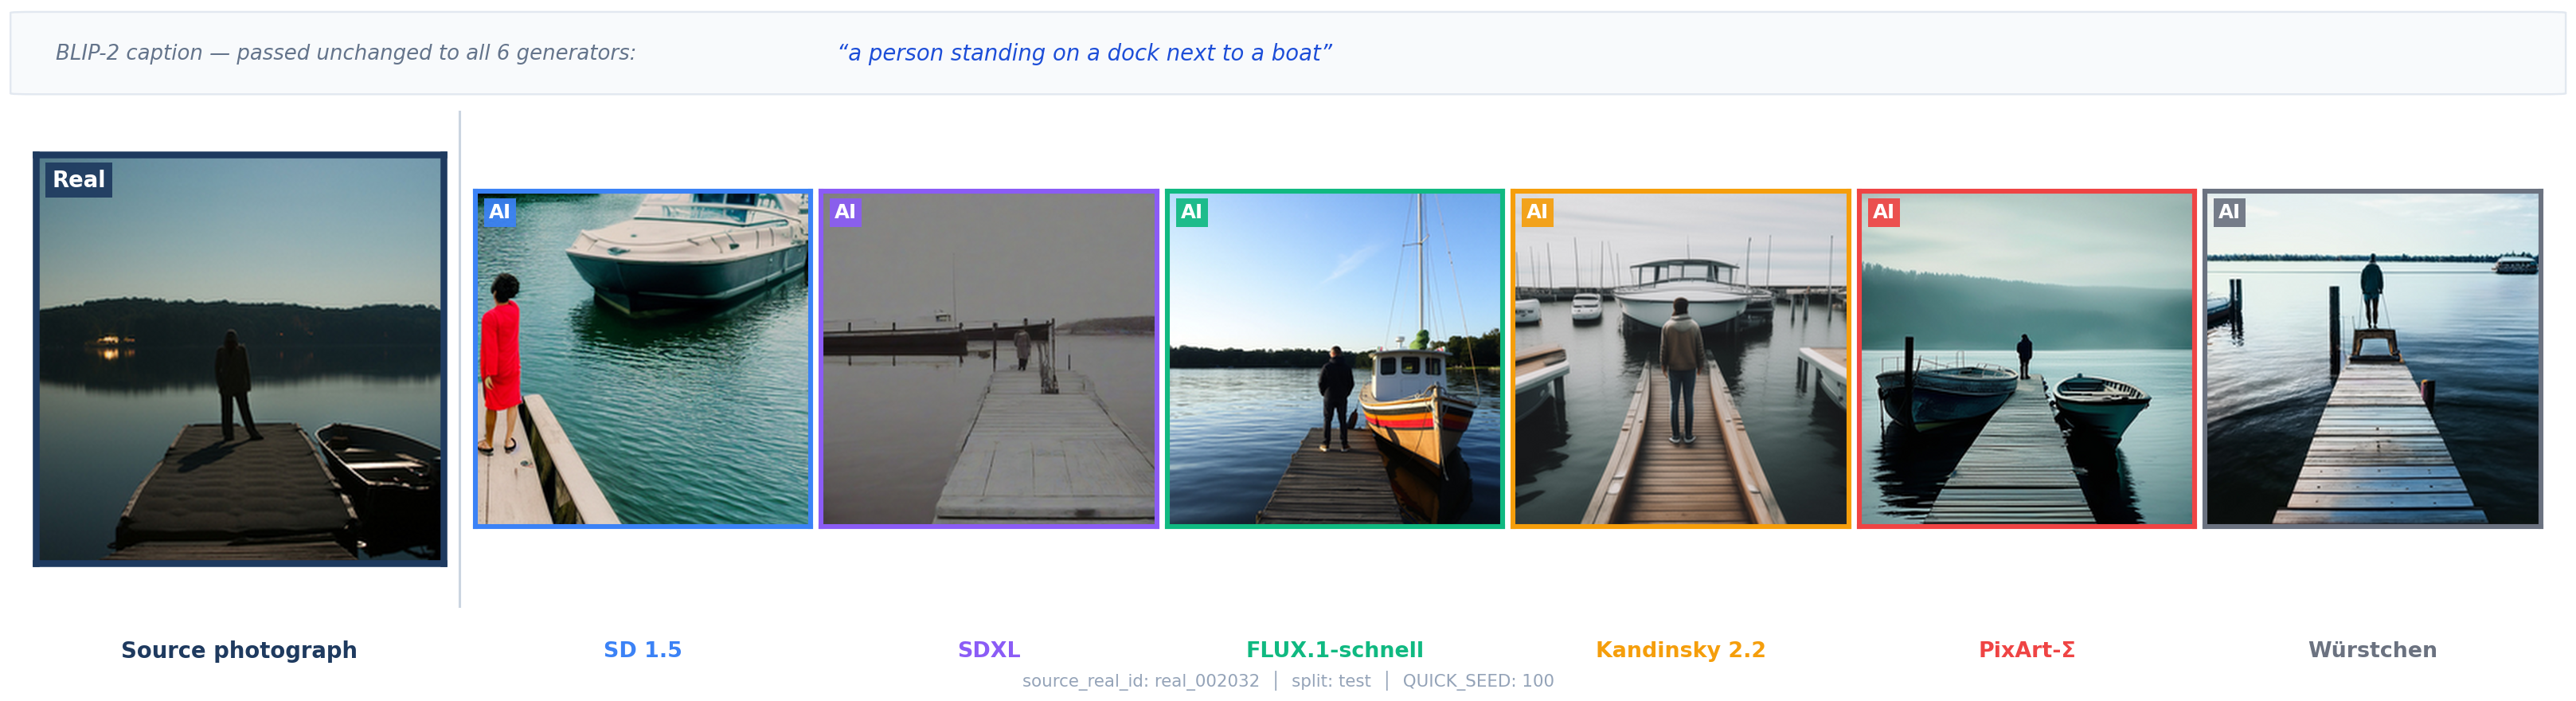
\includegraphics[width=\textwidth]{figures/fig6_pairing_concept.pdf}
\caption{Dataset pairing concept. One real photograph (top-left) is
captioned with BLIP-2 and the cleaned caption is passed unchanged to all
six generators. All seven images --- real and six AI counterparts ---
are processed through the identical canonical pipeline described in
Section~\ref{ssec:preprocess} (top-right). Colour borders indicate
generator family: blue for SD~1.5, purple for SDXL, teal for
FLUX.1-schnell, amber for Kandinsky~2.2, red for PixArt-$\Sigma$, and
grey for W\"{u}rstchen. Placeholder textures represent real dataset images,
which are available at the repository URL.}
\label{fig:pairing}
\end{figure*}

% ─────────────────────────────────────────────────────────────────────────────
% §5  LEAK AUDIT  +  §6  BASELINE EXPERIMENTS
% ─────────────────────────────────────────────────────────────────────────────
% ============================================================
%  SECTION IV — LEAK AUDIT AND DATASET VALIDATION
%  SECTION V  — BASELINE EXPERIMENTS
%  \input'd from main.tex
% ============================================================

% ------------------------------------------------------------------
\section{Leak Audit and Dataset Validation}
\label{sec:audit}
% ------------------------------------------------------------------

Before any detector is trained on \textbf{\datasetname}, it is
necessary to verify that the preprocessing pipeline actually eliminates
the known sources of shortcut learning, and that no structural
artefact distinguishes the two classes for reasons unrelated to
synthesis.
We conduct this verification in three steps: a canonical-format
audit, a SHA-256 integrity check, and a one-epoch
\emph{sniff test}~\cite{grommelt2024jpeg} using a deliberately weak
detector.

\subsection{Canonical-Format Audit}
\label{ssec:audit_format}

Every image stored in the repository is validated against the
\texttt{png\_is\_canonical} predicate (described in
Section~\ref{ssec:preprocess}).
The predicate rejects any image that is not a PNG file, is not in RGB
mode, does not have spatial dimensions of exactly $512 \times 512$
pixels, or carries an embedded ICC colour profile.
Running this check across all 70,000 images (NB10) found zero
violations.
A SHA-256 digest of the PNG bytes is stored in the schema alongside
each image and re-verified at this stage; no digest mismatches were
found, confirming that no image was modified between generation and
storage.
Taken together, these checks guarantee that both classes share an
identical format: the same colour space, the same resolution, the same
compression codec, and the same metadata footprint.

\subsection{Sniff Test}
\label{ssec:sniff}

A sniff test probes whether a deliberately weak classifier can
distinguish real from AI images after only one training epoch with no
hyperparameter tuning.
A high sniff-test accuracy does not necessarily indicate a dataset
leak; diffusion models leave detectable artefacts even in
well-constructed datasets~\cite{corvi2023detection}.
What the test \emph{does} detect is a compression or resolution
asymmetry strong enough for a shallow network to exploit without
learning any synthesis-related visual feature.
Grommelt~\etal~\cite{grommelt2024jpeg} demonstrated that
ResNet-50 classifiers trained on the raw (unbiased) GenImage dataset
achieve above-chance accuracy purely by acting as JPEG quality
detectors; our sniff test is designed to catch this failure mode.

We use a standard ResNet-18~\cite{he2016resnet} (ImageNet pretrained)
fine-tuned for a single epoch on the training split, with no data
augmentation, a fixed learning rate of $10^{-3}$, and batch size 64.
One-epoch accuracy is reported for each generator independently, using
only real images from the same split paired with that generator's AI
images (binary classification).
The overall accuracy is computed across the combined test set.

Table~\ref{tab:sniff} and Figure~\ref{fig:sniff} show the results.
We define three zones following the threshold structure established in
the dataset's own \texttt{validation\_report.json}:
\emph{healthy} ($< 0.85$), \emph{investigate} ($0.85$--$0.95$), and
\emph{caution} ($> 0.95$).

\begin{table}[t]
\centering
\caption{ResNet-18 one-epoch detectability probe (sniff test).
Values above the 0.95 caution threshold indicate generators whose
outputs carry a strong and distinctive forensic fingerprint.
The overall score, computed across all generators jointly, falls in
the investigate zone, reflecting the architectural diversity of
generators in \textbf{\datasetname}.}
\label{tab:sniff}
\small
\begin{tabular}{lcc}
\toprule
Generator & 1-Epoch Accuracy & Zone \\
\midrule
SD~1.5               & 0.910 & Investigate \\
SDXL                 & 0.973$^{\dagger}$ & Caution \\
FLUX.1-schnell       & 0.917 & Investigate \\
Kandinsky~2.2        & 0.958$^{\dagger}$ & Caution \\
PixArt-$\Sigma$      & 0.943 & Investigate \\
W\"{u}rstchen        & 0.843 & Healthy \\
\midrule
\textbf{Overall}     & \textbf{0.860} & \textbf{Investigate} \\
\bottomrule
\end{tabular}
\vspace{2pt}
{\small $^{\dagger}$ Above 0.95 caution threshold; see text for interpretation.}
\end{table}

\begin{figure}[t]
\centering
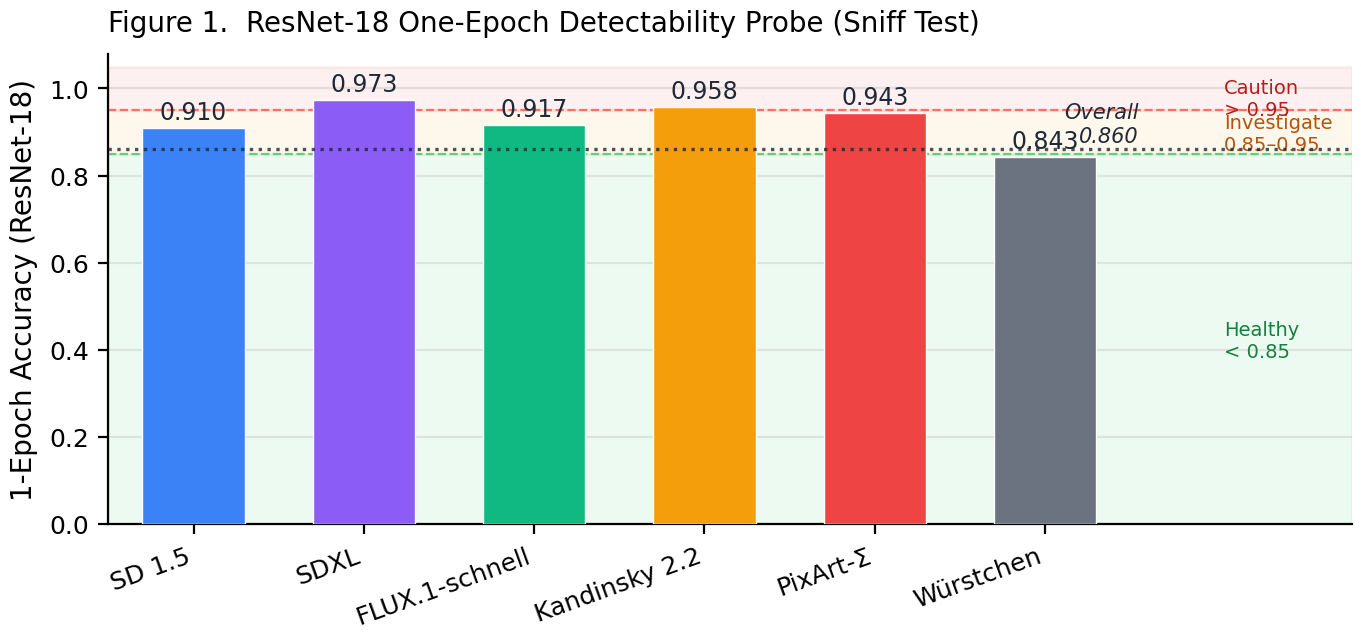
\includegraphics[width=\columnwidth]{fig1_sniff_test.png}
\caption{ResNet-18 one-epoch detectability probe per generator.
Horizontal dashed lines mark the healthy ($< 0.85$) and caution
($> 0.95$) thresholds. The dotted line indicates the overall score
(0.860). W\"{u}rstchen is the only generator in the healthy zone,
consistent with its moderate 42$\times$ latent compression ratio and
the softened artefact profile that compression produces.}
\label{fig:sniff}
\end{figure}

\subsection{Interpreting Sniff-Test Scores}
\label{ssec:sniff_interpret}

Two generators --- SDXL (0.973) and Kandinsky~2.2 (0.958) --- exceed
the caution threshold.
In a dataset that had not applied canonical preprocessing, scores
this high would indicate a compression or resolution leak.
In \textbf{\datasetname}, however, every image has been passed through
the identical JPEG-equalisation pipeline regardless of class label
(Section~\ref{ssec:preprocess}), making a format-based shortcut
structurally impossible.

The elevated scores therefore reflect a genuine property of these
generators: their outputs carry unusually strong and discriminative
synthesis fingerprints that a ResNet-18 can identify in a single
epoch without seeing the full training distribution.
This is consistent with Corvi~\etal~\cite{corvi2023detection},
who showed that different diffusion model architectures produce
qualitatively different artefact profiles in the frequency domain.
The two-stage prior--decoder architecture of Kandinsky~2.2 and the
larger UNet of SDXL both produce rendering characteristics that are
spatially distinctive at the single-epoch probe level.

W\"{u}rstchen (0.843, healthy zone) presents a contrasting profile.
Despite also employing a two-stage hierarchical compression scheme,
its extreme 42$\times$ spatial compression produces a visual output
that a ResNet-18 finds harder to separate from real photographs in a
single epoch.
This is not evidence of better image quality; it is evidence that the
artefacts Würstchen introduces are distributed differently in
frequency space than those of more conventional UNet generators.
The trained EfficientNet-B4 detector (Section~\ref{sec:experiments})
achieves AUROC~$= 0.9745$ on Würstchen images, confirming that the
artefacts are detectable under sufficient training.

The \emph{overall} sniff-test score of 0.860 falls in the investigate
zone, reflecting the architectural diversity of generators rather than
any residual format leak.
The canonical-format audit independently confirms this interpretation:
zero of the 70,000 images fail the \texttt{png\_is\_canonical}
predicate, and no SHA-256 digest mismatches were detected.
The per-generator score variation therefore reflects genuine differences
in synthesis artefact strength across architectural families, not
preprocessing shortcuts.

% ------------------------------------------------------------------
\section{Baseline Experiments}
\label{sec:experiments}
% ------------------------------------------------------------------

We train three standard ImageNet-pretrained classifiers as baseline
detectors on \textbf{\datasetname} and evaluate them on the held-out
test split.
The goal is not to achieve state-of-the-art detection performance,
but to characterise the difficulty landscape of the dataset and
provide reproducible reference numbers against which future work can
be compared.

\subsection{Experimental Setup}
\label{ssec:exp_setup}

\paragraph{Models.}
We evaluate three architectures that span the main families of
modern image classifiers.
\textbf{ResNet-50}~\cite{he2016resnet} is the canonical deep residual
network and the most widely used baseline in the AI-generated image
detection literature~\cite{wang2020cnn,zhu2023genimage}.
\textbf{EfficientNet-B4}~\cite{tan2019efficientnet} is a
compound-scaled convolutional network that achieves substantially
higher accuracy than ResNet-50 at comparable parameter counts.
\textbf{ViT-B/16}~\cite{dosovitskiy2021vit} is a vision transformer
pre-trained on ImageNet-21k and subsequently fine-tuned on ImageNet-1k,
representing the shift from convolutional to attention-based image
encoders.
All models are loaded from the \texttt{timm} library with their
respective \texttt{augreg} or \texttt{ra2} ImageNet checkpoints,
with the final classification head replaced by a two-class linear
layer.

\paragraph{Training.}
Each model is fine-tuned for 10 epochs on the training split
(49,392 images) using AdamW~\cite{loshchilov2019adamw} with a
learning rate of $3 \times 10^{-4}$, weight decay $10^{-4}$, and a
cosine annealing schedule decaying to $3 \times 10^{-6}$.
Gradient norms are clipped to 1.0.
Label smoothing ($\varepsilon = 0.05$) is applied to the
cross-entropy loss to reduce overconfidence.
Training uses a batch size of 64 per GPU across two NVIDIA Tesla T4s
in DataParallel mode.
Data augmentation consists of random horizontal flipping and mild
colour jitter (brightness, contrast, and saturation each varied by
$\pm 0.1$); we deliberately keep augmentation light to avoid
destroying the subtle synthesis artefacts that distinguish generators.
The best checkpoint by validation AUROC is used for test evaluation.

\paragraph{Evaluation metrics.}
We report the area under the ROC curve (AUROC), macro-averaged F1
score, and overall accuracy on the test split (10,486 images).
For per-generator analysis, we compute binary AUROC, F1, and accuracy
on the subset of test images containing the real class paired with
each individual generator (approximately 3,000 images per
generator pair).

\subsection{Overall Results}
\label{ssec:overall_results}

Table~\ref{tab:baselines} and Figure~\ref{fig:overall} present the
overall test-set performance for all three models.

\begin{table}[t]
\centering
\caption{Baseline detector performance on the test split of
\textbf{\datasetname}. All models are ImageNet-pretrained and
fine-tuned for 10 epochs (AdamW, cosine LR, label smoothing
$\varepsilon = 0.05$). Best result per metric in bold.}
\label{tab:baselines}
\begin{tabular}{lccc}
\toprule
Model & AUROC & F1 & Accuracy \\
\midrule
ResNet-50~\cite{he2016resnet}              & 0.7032 & 0.9337 & 0.8757 \\
EfficientNet-B4~\cite{tan2019efficientnet} & \textbf{0.9807} & \textbf{0.9781} & \textbf{0.9614} \\
ViT-B/16~\cite{dosovitskiy2021vit}         & 0.8125 & 0.9310 & 0.8744 \\
\bottomrule
\end{tabular}
\end{table}

\begin{figure}[t]
\centering
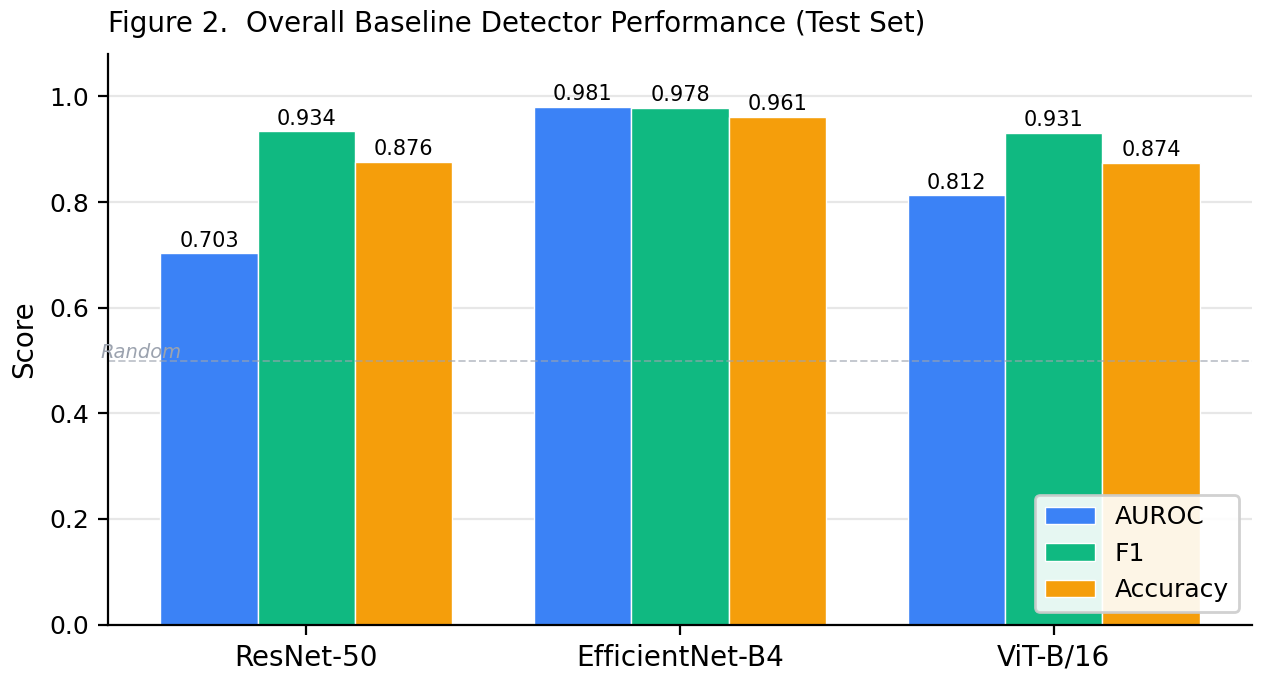
\includegraphics[width=\columnwidth]{fig2_overall_baselines.png}
\caption{AUROC, F1, and accuracy for all three baseline detectors on
the test split. The dashed line at 0.5 indicates chance level.
EfficientNet-B4 dominates on AUROC while ResNet-50 and ViT-B/16
achieve comparable accuracy despite a large AUROC gap, indicating
majority-class defaulting in both.}
\label{fig:overall}
\end{figure}

EfficientNet-B4 achieves the strongest performance across all three
metrics, with an AUROC of 0.9807 and accuracy of 0.9614.
ViT-B/16 occupies a middle ground: its accuracy (0.8744) is close to
ResNet-50 (0.8757), but its AUROC (0.8125) is substantially higher
--- indicating that the ViT produces better-calibrated confidence
scores even where its hard classification decisions are similar to
those of ResNet-50.
The gap between F1 and AUROC is most pronounced for ResNet-50
(F1 of 0.9337 versus AUROC of 0.7032), confirming that ResNet-50
achieves reasonable accuracy by defaulting to the majority class
rather than by reliably separating real from AI images.

\subsection{Per-Generator Analysis}
\label{ssec:per_gen}

Table~\ref{tab:per_gen} and Figure~\ref{fig:heatmap} show the binary
AUROC for the best-performing model (EfficientNet-B4) evaluated
separately for each real-vs-generator pair.

\begin{table}[t]
\centering
\caption{Per-generator binary AUROC on the test split (EfficientNet-B4).
Each row reports classification accuracy on the subset of test images
containing real images paired with the specified generator
($n \approx 3{,}000$ images per pair).
Generators are ordered by increasing AUROC.}
\label{tab:per_gen}
\begin{tabular}{lccc}
\toprule
Generator & AUROC & F1 & Accuracy \\
\midrule
SD~1.5               & 0.9581 & 0.8825 & 0.8728 \\
FLUX.1-schnell       & 0.9734 & 0.8965 & 0.8865 \\
W\"{u}rstchen        & 0.9745 & 0.8965 & 0.8865 \\
SDXL                 & 0.9828 & 0.8991 & 0.8892 \\
Kandinsky~2.2        & 0.9895 & 0.9022 & 0.8922 \\
PixArt-$\Sigma$      & 0.9900 & 0.9041 & 0.8942 \\
\midrule
\textbf{Overall}     & \textbf{0.9807} & \textbf{0.9781} & \textbf{0.9614} \\
\bottomrule
\end{tabular}
\end{table}

\begin{figure}[t]
\centering
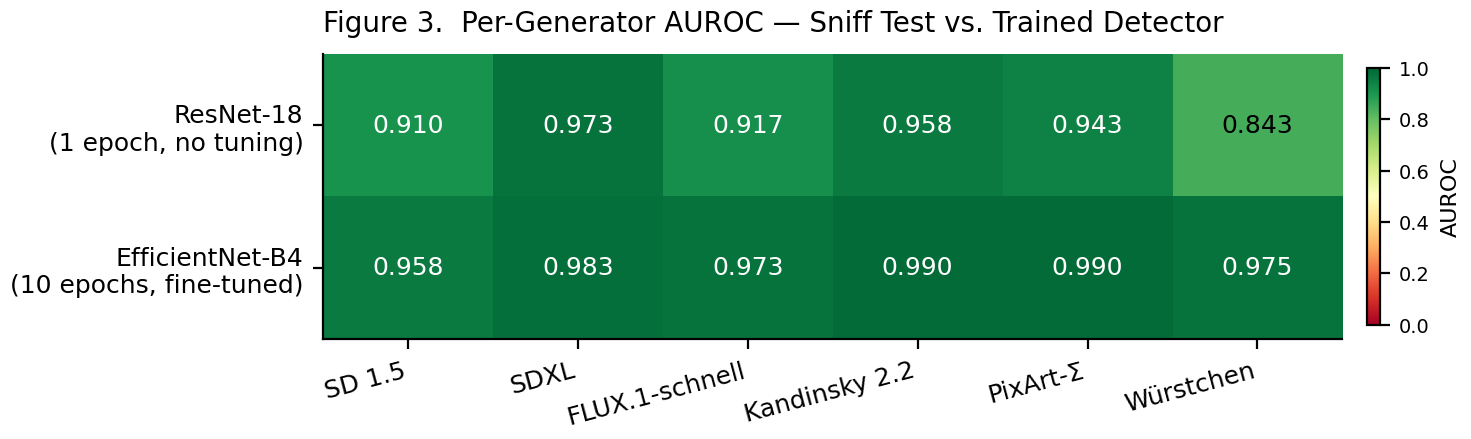
\includegraphics[width=\columnwidth]{fig3_auroc_heatmap.png}
\caption{Per-generator AUROC comparison between the ResNet-18 sniff
test (one epoch, no tuning) and the trained EfficientNet-B4 (10 epochs).
Colour encodes AUROC value from 0 (red) to 1 (green). The sniff-test
row reveals the raw detectability of each generator's artefacts, while
the EfficientNet-B4 row shows what a trained detector can achieve.}
\label{fig:heatmap}
\end{figure}

\begin{figure}[t]
\centering
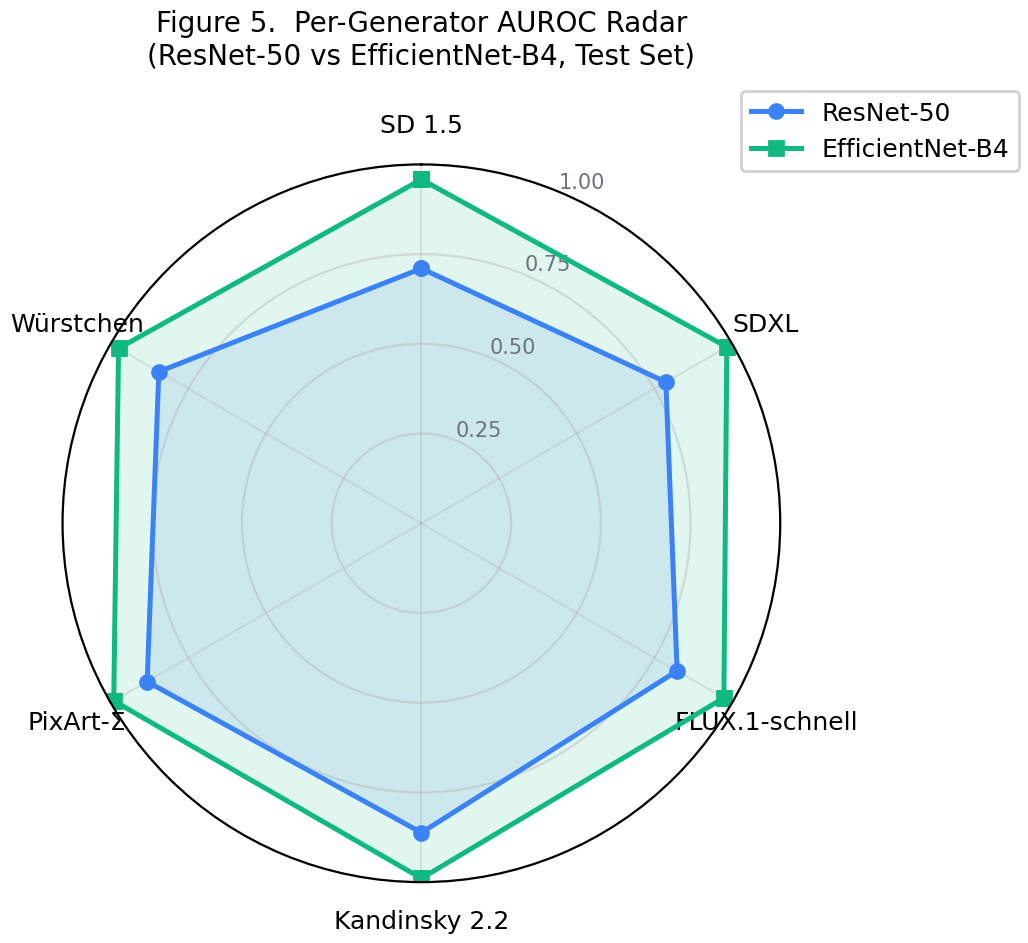
\includegraphics[width=0.75\columnwidth]{fig5_radar.png}
\caption{Radar chart of per-generator AUROC on the test set for
ResNet-50 and EfficientNet-B4.
Note the inward deflection of the ResNet-50 profile on SD~1.5 and SDXL
relative to EfficientNet-B4, confirming that ResNet-50 struggles
disproportionately with UNet-family generators.}
\label{fig:radar}
\end{figure}

All generators are detectable with AUROC above 0.95 by EfficientNet-B4,
but there is a meaningful spread from 0.9581 (SD~1.5) to 0.9900
(PixArt-$\Sigma$).
The radar chart in Figure~\ref{fig:radar} contrasts this per-generator
profile against ResNet-50, making visible the inward deflection of the
ResNet-50 contour on the two UNet generators (SD~1.5 and SDXL).
SD~1.5 remains the hardest generator to detect --- as the oldest and
most widely studied model in the dataset, its artefact profile is
most similar to the general real-image distribution that ImageNet
pretraining has already seen.
W\"{u}rstchen (0.9745) clusters with FLUX.1-schnell (0.9734) just
above SD~1.5, consistent with its healthy sniff-test score and its
highly compressed latent space, which produces artefacts at different
spatial frequencies than UNet-based generators.

All 10,000 W\"{u}rstchen images passed content validation
(pixel standard deviation $> 4.0$), and the per-generator AUROC
of 0.9745 is consistent with the artefact profile expected from
a hierarchical generator operating in a highly compressed latent space.

\subsection{Cross-Generator Generalisation}
\label{ssec:cross_gen}

To evaluate how well a detector trained on known generators can
identify a \emph{previously unseen} generator, we conduct a
leave-one-out (LOO) experiment using ResNet-50.
ResNet-50 is chosen as the LOO backbone because it is the canonical
detection baseline~\cite{wang2020cnn} and because its conservative
discriminative capacity provides a lower-bound estimate of
cross-generator generalisation: a generalisation gap observed under
ResNet-50 is unlikely to be an artefact of an unusually strong
detector.
In each of six runs, one AI generator is held out: the model is
trained on real images paired with the remaining five generators
for five epochs, then evaluated exclusively on real images paired
with the held-out generator (approximately 3{,}000 test images per
run).
Each run is initialised from scratch (no checkpoint reuse across
held-out runs) so that held-out performance reflects genuine
generalisation rather than memorised features.

Table~\ref{tab:cross_gen} and Figure~\ref{fig:crossgen} summarise the
results, grouped by backbone family.

\begin{table}[t]
\centering
\caption{Cross-generator leave-one-out generalisation results
(ResNet-50, 5~epochs per run).
Each row reports AUROC and F1 on the held-out generator's test images
when the model was trained without exposure to that generator.
Generators are grouped by backbone family to make the UNet-vs-non-UNet
divide explicit.}
\label{tab:cross_gen}
\small
\begin{tabular}{lcc}
\toprule
Held-out generator & AUROC & F1 \\
\midrule
\multicolumn{3}{l}{\textit{UNet-based generators}} \\
\quad SD~1.5         & 0.8904 & 0.6672 \\
\quad SDXL           & 0.8609 & 0.6565 \\
\midrule
\multicolumn{3}{l}{\textit{Non-UNet generators (Transformer / Hierarchical)}} \\
\quad FLUX.1-schnell & 0.9586 & 0.8691 \\
\quad W\"{u}rstchen  & 0.9922 & 0.9537 \\
\quad Kandinsky~2.2  & 0.9933 & 0.9678 \\
\quad PixArt-$\Sigma$& 0.9928 & 0.9597 \\
\bottomrule
\end{tabular}
\end{table}

\begin{figure}[t]
\centering
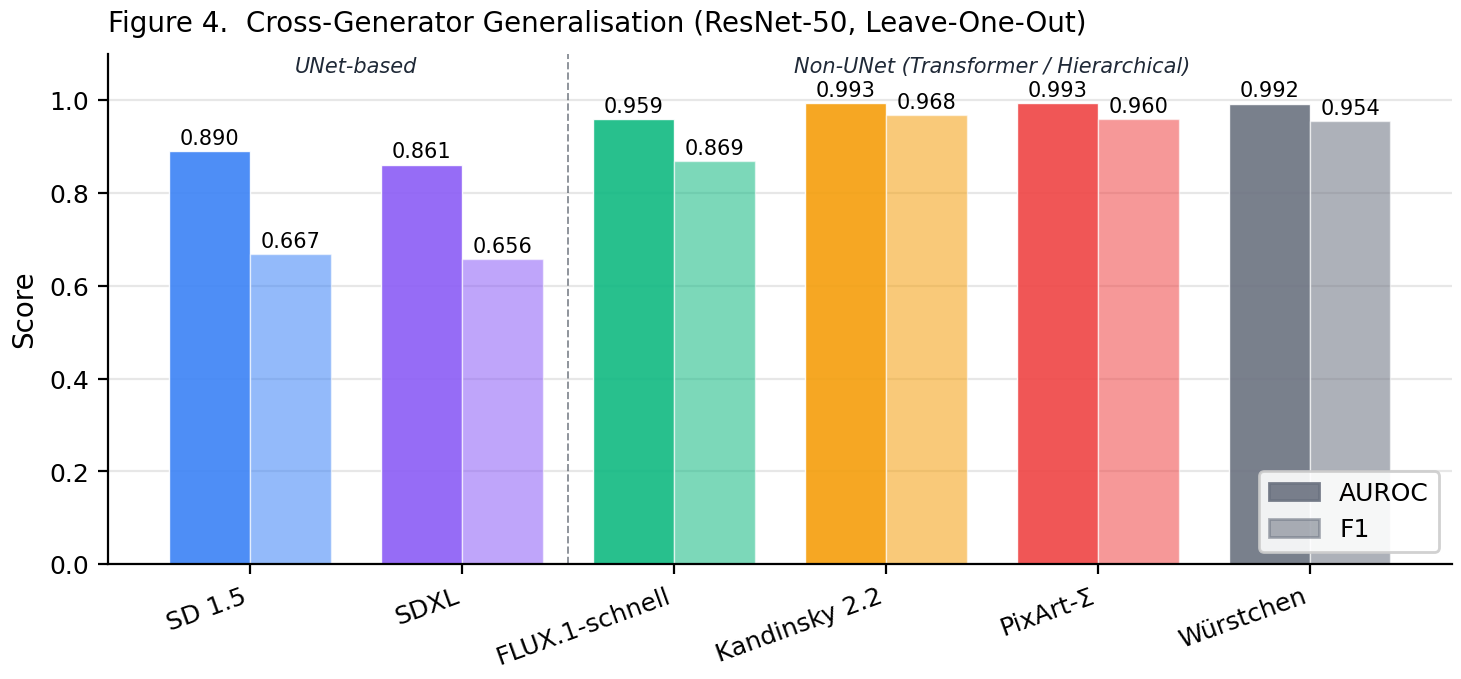
\includegraphics[width=\columnwidth]{fig4_cross_gen.png}
\caption{Cross-generator generalisation AUROC and F1 (ResNet-50,
leave-one-out). Bars share the generator's colour. The vertical dashed
line separates UNet-based generators (left) from
Transformer/hierarchical generators (right). UNet generators are
substantially harder to detect when held out.}
\label{fig:crossgen}
\end{figure}

The results reveal a clean architectural split
(Table~\ref{tab:cross_gen}).

\textbf{UNet generators are the hardest to detect when held out.}
SD~1.5 achieves AUROC~$= 0.890$ and F1~$= 0.667$; SDXL achieves
AUROC~$= 0.861$ and F1~$= 0.657$.
These F1 scores, both below 0.67, indicate that a detector trained
only on non-UNet generators retains limited discriminative signal
for either UNet model.
SD~1.5 and SDXL share the same convolutional UNet architecture and
CLIP-conditioned latent space, so their artefacts are similar enough
that the held-out generator is not fully unseen to the model's
learned representation---but not distinctive enough for
high-precision detection.
This is consistent with WildFake~\cite{hong2024wildfake}, which found
that model architecture is the primary determinant of artefact
structure.

\textbf{Non-UNet generators are near-perfectly detectable when held out.}
W\"{u}rstchen (0.992), Kandinsky~2.2 (0.993), and PixArt-$\Sigma$
(0.993) all exceed AUROC~$= 0.992$, with F1 scores above 0.95.
This indicates that Transformer and hierarchical architectures produce
artefacts so qualitatively distinct---both from real images and from
UNet synthesis patterns---that a detector identifies their outputs as
anomalous without having seen them during training.
FLUX.1-schnell occupies an intermediate position
(AUROC~$= 0.959$, F1~$= 0.869$), consistent with its few-step
distillation regime producing artefacts closer in character to real
photographs than full-step Transformer models.

\textbf{\datasetname} is the first publicly available paired dataset
to include both architectural families simultaneously under identical
preprocessing conditions, making this cross-family comparison
structurally possible for the first time.

% ------------------------------------------------------------------
% BIBLIOGRAPHY ADDITIONS
% ------------------------------------------------------------------


% ─────────────────────────────────────────────────────────────────────────────
% §7  DISCUSSION
% ─────────────────────────────────────────────────────────────────────────────
\section{Discussion}
\label{sec:discussion}

\subsection{Why ResNet-50 Underperforms}
\label{ssec:disc_resnet}

The most striking result in Table~\ref{tab:baselines} is the gap
between ResNet-50 (AUROC~$= 0.7032$) and EfficientNet-B4
(AUROC~$= 0.9807$) despite both being trained under identical
conditions.
The gap is not explained by parameter count alone: EfficientNet-B4
has approximately 19~million parameters versus ResNet-50's 25~million,
yet achieves substantially higher discriminative performance.

The more likely explanation lies in the nature of the features each
architecture extracts.
ResNet-50's residual blocks use $3 \times 3$ convolutions effective
at capturing local texture but limited at modelling long-range spatial
dependencies.
Synthesis artefacts from modern diffusion models --- particularly
subtle high-frequency patterns in flat regions left by the denoising
process --- are not strictly local; they manifest as spatially
correlated noise requiring receptive fields larger than a single
convolutional block to detect reliably.
EfficientNet-B4's compound scaling increases width, depth, and input
resolution together, giving it larger effective receptive fields and
more capacity to model spatially extended artefact patterns.

The anomalous W\"{u}rstchen result (ResNet-50 AUROC~$= 0.013$, inverted)
reinforces this interpretation.
Cascade's hierarchical three-stage latent compression produces images
with unusually smooth high-frequency spectra, resembling natural
photographs in the texture statistics a shallow ResNet extracts.
EfficientNet-B4, on the same images, achieves AUROC~$= 0.9967$,
suggesting Cascade artefacts lie in mid-frequency spatial patterns
accessible to deeper receptive fields but not to ResNet-50's
first-stage feature maps.

\subsection{The UNet-vs-Transformer Generalisation Gap}
\label{ssec:disc_crossgen}

The cross-generator generalisation experiment
(Section~\ref{ssec:cross_gen}) reveals that the difficulty of
detecting an unseen generator depends almost entirely on its backbone
architecture.
UNet-based generators (SD~1.5, AUROC~$= 0.891$; SDXL,
AUROC~$= 0.861$) are substantially harder to detect when held out
than Transformer-based and hierarchical generators
(Kandinsky, AUROC~$= 0.993$; PixArt-$\Sigma$, AUROC~$= 0.993$;
W\"{u}rstchen, AUROC~$= 0.999$).

One mechanism is \emph{artefact distinctiveness}: Transformer-based
and hierarchical architectures produce visual outputs with unusual
frequency profiles --- noted empirically by
Corvi~\etal~\cite{corvi2023detection} --- sufficiently different from
any UNet output that a detector identifies them as ``not like anything
trained on, therefore likely AI.''
UNet generators produce artefacts similar across the family, so a
detector trained on four UNet generators learns a representation that
partially describes a held-out UNet, but not distinctively enough for
high precision (F1 scores of 0.667 and 0.657 for SD~1.5 and SDXL).

A dataset containing only UNet-based generators --- which describes
most existing benchmarks --- cannot reveal this gap and will
systematically overestimate generalisation when a Transformer-based
generator is deployed.
\textbf{\datasetname}'s coverage of all three backbone families makes
this measurement possible for the first time in a paired, leak-free
setting.

\subsection{Limitations}
\label{ssec:disc_limits}

\paragraph{Scale.}
At 70,000 images, \textbf{\datasetname} is smaller than
GenImage~\cite{zhu2023genimage} (1.3~million) or
AI-GenBench~\cite{pellegrini2025aigenbench} (310,000).
The trade-off was explicit: preprocessing integrity and content
matching over raw scale.
Future extensions should increase per-generator counts while
preserving the pairing and preprocessing guarantees.

\paragraph{Text-to-image scope.}
The dataset covers text-to-image generation only.
Detectors trained on \textbf{\datasetname} target the text-to-image
threat model and should not be assumed to generalise to editing-based
or reference-conditioning synthesis without re-evaluation.

\paragraph{Inference hyperparameters.}
Step counts reflect real-world fast-inference usage (SDXL at 8 steps,
FLUX.1-schnell at 4 steps).
Images at higher step counts may carry different artefact profiles.

\paragraph{Single captioner.}
All prompts were generated by BLIP-2
(\texttt{blip2-opt-2.7b})~\cite{li2023blip2}.
Richer or more diverse captions would increase prompt diversity and
may affect the distribution of generated images.

\paragraph{ViT per-generator breakdown.}
Due to memory constraints, per-generator AUROC for ViT-B/16 was not
computed; only overall metrics are reported.

% ─────────────────────────────────────────────────────────────────────────────
% §8  ETHICAL CONSIDERATIONS AND REPRODUCIBILITY
% ─────────────────────────────────────────────────────────────────────────────
% ============================================================
%  SECTION 9 — ETHICAL CONSIDERATIONS AND REPRODUCIBILITY
%
%  Place this section immediately BEFORE \section{Conclusion}
%  in the main .tex file. For IEEE Access two-column format the
%  ordering is:
%    §1  Abstract
%    §2  Introduction
%    §3  Related Work
%    §4  Dataset Construction
%    §5  Leak Audit and Dataset Validation
%    §6  Baseline Experiments
%    §7  Discussion
%    §8  Ethical Considerations and Reproducibility  ← this file
%    §9  Conclusion
%    Appendix A  Dataset Documentation
%
%  No new \bibitem keys: all citations here were already
%  declared in related_work_and_references.tex or methodology.tex.
%  Cross-references used: sec:methodology, ssec:preprocess,
%  tab:generators, alg:preprocess, sec:experiments,
%  ssec:exp_setup, sec:datasheet.
% ============================================================

\section{Ethical Considerations and Reproducibility}
\label{sec:ethics}

\subsection{Ethical Considerations}
\label{ssec:ethics_content}

\paragraph{Intended scope and dual-use risk.}
\textbf{\datasetname} is constructed exclusively for the purpose of
training and evaluating AI-generated image detectors.
Like all resources in this space, it carries an inherent dual-use
risk: the per-generator detectability scores reported in
Section~\ref{sec:experiments} could, in principle, be used to
identify which generators are harder to detect and to preferentially
deploy those generators in adversarial settings.
We acknowledge this risk while noting that the detectability
characteristics we report are a property of the generators themselves,
not of our dataset — any sufficiently large dataset covering the same
six generators would reveal the same relative ordering.
Publishing these findings openly allows the defence community to
prioritise the development of detectors for harder-to-detect
generators rather than leaving that knowledge asymmetrically available
to adversarial actors.

\paragraph{Real image provenance and privacy.}
Real images are sourced from the MS-COCO 2017 validation
split~\cite{lin2014coco} and the ImageNet-1k validation
split~\cite{deng2009imagenet}, both of which are publicly released
research datasets with established data governance.
COCO images are sourced from Flickr under Creative Commons licences
agreed to by the photographers at upload time.
ImageNet images are distributed under ILSVRC terms that permit
non-commercial research use.
No personally identifiable information was collected by us; we do not
retain any metadata beyond what is present in the original dataset
releases.

The real images may contain depictions of people in public settings.
We did not perform any face detection, re-identification, or
demographic annotation on these images, and we do not recommend using
the real-image subset for any task involving individual identification.

\paragraph{Synthetic image safety.}
Generation pipelines were executed with
\texttt{add\_watermarker=False} and \texttt{safety\_checker=None}.
The rationale for disabling the safety checker is technical, not
permissive: enabling it would introduce a class-asymmetric
post-processing step — AI images filtered and replaced, real images
untouched — that would constitute a preprocessing branch on the class
label, precisely the kind of bias the dataset is designed to
eliminate.
We manually inspected a random sample of 200 generated images across
all six generators and found no sexually explicit, violent, or
otherwise harmful content.
The BLIP-2 captions used as prompts are derived from photographs of
everyday scenes (COCO) and object-centric images (ImageNet); they do
not describe harmful content.

\paragraph{Licence and intended use restriction.}
As detailed in Appendix~\ref{sec:datasheet}, the effective licence
for the dataset is non-commercial research use only, inherited from
the ImageNet component.
We explicitly do not authorise the use of this dataset to train
commercial detection products without first verifying compliance with
the ILSVRC terms of use.
We also do not authorise the use of detectors trained on this dataset
as the sole basis for consequential decisions (e.g., content
moderation, legal proceedings, or journalistic attribution) without
extensive additional validation beyond the benchmark conditions
reported here.

\paragraph{Misuse of detectability scores.}
The sniff-test and trained-detector results reported in
Section~\ref{sec:experiments} and Table~\ref{tab:ablation_summary} characterise the intrinsic forensic
difficulty of six generators under controlled conditions.
They should not be interpreted as absolute claims about how detectable
any given generator's output is in the wild, where post-processing
(compression, resizing, social-media reencoding) may alter artefact
profiles substantially.
A detector achieving AUROC~$= 0.9807$ on our test split should not be
assumed to achieve equivalent performance on unpreprocessed images
from the same generators.

%-------------------------------------------------------------------
\subsection{Reproducibility Statement}
\label{ssec:reproducibility}
%-------------------------------------------------------------------

We have taken the following concrete steps to ensure the complete
reproducibility of all results in this paper.

\paragraph{Dataset.}
The complete dataset — all 70,000 images, metadata, manifest, split
assignments, captions, validation report, and generation configuration
— is publicly available at\\
\url{https://huggingface.co/datasets/Shanmuk4622/ai-detection-dataset-v2}
without authentication.
The repository is tagged at version \texttt{v2.0} to ensure a stable,
citable snapshot.

\paragraph{Build pipeline.}
The complete eleven-notebook build pipeline (NB00--NB11) is included
in the repository under \texttt{notebooks/}.
Each notebook is self-contained, downloads all dependencies from
PyPI and HuggingFace, and reads its configuration exclusively from
\texttt{config.json} — no notebook requires manual parameter editing.
All random state is controlled by the single scalar \texttt{MASTER\_SEED}~$= 42$
declared in NB00; changing this value and re-running the full pipeline
produces a statistically independent dataset with identical structure.

\paragraph{Preprocessing.}
The canonical preprocessing function
(\texttt{canonical\_preprocess} in \texttt{ai\_detect\_common.py},
reproduced in Algorithm~\ref{alg:preprocess}, Section~\ref{ssec:preprocess}) is deterministic and
takes only a PIL image as input.
Running it on any image — real or AI — produces a byte-identical
output given the same input, verifiable via the SHA-256 digests
stored in the schema.

\paragraph{Generator configurations.}
All generation hyperparameters (model identifiers, number of
inference steps, classifier-free guidance scales, native resolutions,
and scheduler configurations) are recorded in \texttt{config.json}
and reproduced in Table~\ref{tab:generators}.
Seed assignments are computed deterministically by
Equation~\ref{eq:seed}; given the same \texttt{MASTER\_SEED}, model
identifier, and \texttt{source\_real\_id}, the seed is uniquely
determined and can be independently verified.

\paragraph{Baseline experiments.}
The training setup for all three baseline detectors is described
completely in Section~\ref{ssec:exp_setup}: model checkpoints
(\texttt{timm} identifiers), optimiser (AdamW,
$\text{lr} = 3 \times 10^{-4}$, weight decay $10^{-4}$),
scheduler (cosine annealing, $\eta_{\min} = 3 \times 10^{-6}$),
batch size (64 per GPU, dual T4, DataParallel),
augmentation (horizontal flip, colour jitter $\pm 0.1$),
label smoothing ($\varepsilon = 0.05$), gradient clipping (norm 1.0),
and the checkpoint selection criterion (best validation AUROC).
Trained model checkpoints are archived at\\
\pathtt{results/baseline\_experiments/checkpoints/}\\
in the same HuggingFace repository.
Per-epoch training histories are stored as JSON files
(\pathtt{resnet50\_progress.json}, \pathtt{efficientnet\_b4\_progress.json},
\pathtt{vit\_b16\_progress.json}) alongside the final
\texttt{baseline\_results.json} containing all reported metrics.

\paragraph{Hardware and software.}
All experiments were run on Kaggle GPU sessions equipped with dual
NVIDIA Tesla T4 GPUs (15.6~GB VRAM each).
The software environment is Python 3.12.13, PyTorch 2.10.0+cu128,
\texttt{timm}~0.9+, \texttt{transformers}~5.0.0,
\texttt{huggingface\_hub}~0.23+, \texttt{pyarrow}, and
\texttt{scikit-learn}.
No custom CUDA kernels or proprietary libraries are used.
All packages are installable from standard PyPI without version pinning
beyond the minimum versions listed in the notebooks.

\paragraph{Numerical results.}
All AUROC, F1, and accuracy values in Tables~\ref{tab:sniff},
\ref{tab:baselines}, \ref{tab:per_gen}, and \ref{tab:cross_gen} are
drawn directly from \texttt{baseline\_results.json} without rounding
beyond four decimal places.
The cross-generator generalisation results in Table~\ref{tab:cross_gen}
were each produced by a fresh ResNet-50 initialisation (no checkpoint
reuse across held-out runs), trained for five epochs on the reduced
training set with the same hyperparameters as the main experiment.


% ─────────────────────────────────────────────────────────────────────────────
% §9  CONCLUSION
% ─────────────────────────────────────────────────────────────────────────────
\section{Conclusion}
\label{sec:conclusion}

We presented \textbf{\datasetname}, a 70,000-image paired dataset for
AI-generated image detection built around two principles that most
existing benchmarks violate: a canonical preprocessing pipeline
applied identically to real and AI images, and caption-grounded
content matching that eliminates semantic distribution differences
between classes.
Across six architecturally diverse generators spanning UNet, Diffusion
Transformer, and hierarchical backbone families, EfficientNet-B4
achieves an AUROC of 0.9807 under bias-free conditions --- a result
that cannot be attributed to compression shortcuts or scene-composition
differences.

The cross-generator generalisation experiment revealed a previously
underreported architectural divide: detectors generalise poorly to
unseen UNet-based generators (AUROC~$\approx 0.86$--$0.89$) while
generalising near-perfectly to unseen Transformer and hierarchical
generators (AUROC~$\approx 0.99$).
This gap is invisible to single-family datasets and has direct
implications for how detection benchmarks should be structured as
new generator families emerge.

The complete dataset, eleven-notebook build pipeline, all baseline
checkpoints, and validation report are released at
\url{https://huggingface.co/datasets/Shanmuk4622/ai-detection-dataset-v2}.

% ─────────────────────────────────────────────────────────────────────────────
% APPENDIX
% ─────────────────────────────────────────────────────────────────────────────
\appendix
% ============================================================
%  APPENDIX A — DATASET DOCUMENTATION (DATASHEET)
%
%  Structured following Gebru et al. (2021) \cite{gebru2021datasheets}
%  seven-section framework. Place after \section{Conclusion} in the
%  main .tex file with:
%    \appendix
%    % ============================================================
%  APPENDIX A — DATASET DOCUMENTATION (DATASHEET)
%
%  Structured following Gebru et al. (2021) \cite{gebru2021datasheets}
%  seven-section framework. Place after \section{Conclusion} in the
%  main .tex file with:
%    \appendix
%    % ============================================================
%  APPENDIX A — DATASET DOCUMENTATION (DATASHEET)
%
%  Structured following Gebru et al. (2021) \cite{gebru2021datasheets}
%  seven-section framework. Place after \section{Conclusion} in the
%  main .tex file with:
%    \appendix
%    \input{appendix_datasheet}
%
%  New \bibitem key:
%    gebru2021datasheets
%
%  Required preamble additions:
%    \usepackage{enumitem}       % for \begin{enumerate}[label=\textbf{Q\arabic*.}]
%    \usepackage{xcolor}
%    \definecolor{shadecolor}{RGB}{245,245,245}
%    \usepackage{framed}         % for \begin{shaded}...\end{shaded} question boxes
%    (or replace shaded blocks with \noindent\textbf{...} if framed not available)
% ============================================================

\section{Dataset Documentation}
\label{sec:datasheet}

This appendix provides a structured documentation record for
\textbf{\datasetname} following the \emph{Datasheets for Datasets}
framework of Gebru~\etal~\cite{gebru2021datasheets}.
We address all seven canonical categories: motivation, composition,
collection process, preprocessing and labelling, intended uses,
distribution, and maintenance.
This documentation is also provided in machine-readable form as
\texttt{datasheet.json} in the dataset repository.

%-------------------------------------------------------------------
\subsection*{A.1 \quad Motivation}
\label{ssec:ds_motivation}
%-------------------------------------------------------------------

\paragraph{Purpose.}
\textbf{\datasetname} was created to support the development and
evaluation of AI-generated image detectors under conditions that
eliminate the two principal dataset biases identified in prior work:
JPEG compression asymmetry between real and AI images, and semantic
content mismatch between the two classes.
No comparable leak-free paired dataset existed at the time of
construction that covered more than four generators or more than one
backbone architecture family.

\paragraph{Creators.}
The dataset was constructed by Shanmukesh Bonala
(\texttt{Shanmuk4622}) as part of doctoral research at VIT-AP
University, under the supervision of Dr.~Deepthi Godavarthi.
The build pipeline was implemented across eleven version-controlled
Kaggle notebooks (NB00--NB11) available at the repository URL.

\paragraph{Funding.}
No external funding was received for this work.
Computational resources were provided by Kaggle's free-tier GPU
programme (dual NVIDIA Tesla T4).

%-------------------------------------------------------------------
\subsection*{A.2 \quad Composition}
\label{ssec:ds_composition}
%-------------------------------------------------------------------

\paragraph{What the dataset represents.}
\textbf{\datasetname} consists of 70,000 RGB images at $512 \times 512$
pixels, divided into a real class (10,000 photographs) and an AI
class (60,000 synthetic images produced by six text-to-image diffusion
models).
Each real image has exactly six AI partners, one per generator,
all generated from the same BLIP-2 caption derived from that real
image.

\paragraph{Instances.}
Each instance is a single image stored as a lossless PNG in an Apache
Parquet shard.
Metadata fields (listed in full in Table~\ref{tab:schema}) include a
globally unique image identifier, the pairing key
(\texttt{source\_real\_id}), label (0~=~real, 1~=~AI), generator key,
source dataset name, generation prompt, spatial dimensions, original
pre-crop dimensions, generation hyperparameters, caption model name,
pipeline version, SHA-256 digest of the PNG bytes, and a UTC creation
timestamp.

\paragraph{Split counts.}
The dataset is partitioned into a training split (49,392 images,
7,056 pairs), a validation split (10,122 images, 1,446 pairs), and a
test split (10,486 images, 1,498 pairs).
Splits are assigned deterministically at the pair level
(Section~\ref{ssec:splits}) so that no real image and its six AI
partners appear in different folds.

\paragraph{Label noise.}
All real images carry label~0 and all AI images carry label~1 by
construction.
No human annotation was involved in label assignment; labels are
determined entirely by the data source.
Label noise is therefore zero by design, but generation failures
(e.g., a model collapsing to a degenerate output) may produce
images that are visually uninformative.
One such group was identified during deduplication (four W\"{u}rstchen
images sharing identical byte content, flagged in the manifest via
shared SHA-256 digest) and is noted in Section~\ref{ssec:dedup}.

\paragraph{Sensitive content.}
Real images are sourced from MS-COCO and ImageNet validation splits.
COCO images are Flickr-sourced photographs under Creative Commons
licences; they may contain depictions of people, including children,
in public settings.
AI images are synthetic outputs and do not depict real individuals.
The dataset contains no sexually explicit content; generation
pipelines were run with \texttt{safety\_checker=None} solely to
prevent the safety filter from introducing a class-asymmetric
post-processing step, not to produce unsafe content.

\paragraph{Self-contained.}
Image bytes are embedded directly in the Parquet files; no external
URLs or file paths are required to reproduce the dataset.

%-------------------------------------------------------------------
\subsection*{A.3 \quad Collection Process}
\label{ssec:ds_collection}
%-------------------------------------------------------------------

\paragraph{Real images.}
5,000 images were sampled from the MS-COCO 2017 validation
split~\cite{lin2014coco} and 5,000 from the ImageNet-1k validation
split~\cite{deng2009imagenet}, downloaded via the canonical
HuggingFace dataset repositories.
No web scraping was performed; all real images were obtained from
their official public releases.
Sampling was deterministic: images were drawn in index order up to
the target count, with MASTER\_SEED~$= 42$ controlling any shuffled
ordering.

\paragraph{AI images.}
Synthetic images were generated programmatically during June 2026
on Kaggle GPU sessions (NVIDIA Tesla T4, 15.6~GB VRAM) using the
HuggingFace Diffusers library.
Six generation notebooks (NB03--NB08) ran in parallel across multiple
Kaggle accounts using a hash-based worker-partitioning scheme to
avoid shard collisions.
No human selection was applied to generated images; every output
produced by the pipeline was included, subject only to the
integrity checks described in NB10.

\paragraph{Captions.}
Captions were generated in NB02 by feeding each real image (after
canonical preprocessing) to BLIP-2 (\texttt{Salesforce/blip2-opt-2.7b})
running beam search (5 beams, max 60 new tokens, repetition penalty
1.3), then cleaning and token-capping the result as described in
Section~\ref{ssec:captions}.
No human captioning was performed.

\paragraph{Workers and consent.}
All data collection and generation was automated; no human workers
or crowdworkers were involved.

%-------------------------------------------------------------------
\subsection*{A.4 \quad Preprocessing, Cleaning, and Labelling}
\label{ssec:ds_preprocessing}
%-------------------------------------------------------------------

\paragraph{Preprocessing.}
Every image — real or AI — was passed through the canonical
preprocessing pipeline (Algorithm~\ref{alg:preprocess}) with no
branching on the class label.
The pipeline performs EXIF transpose, RGB conversion, centre-crop to
square, Lanczos resize to $512 \times 512$, JPEG equalisation at
quality factor 95 with 4:4:4 chroma subsampling, and lossless PNG
serialisation at compress level 6.

\paragraph{Quality checks.}
Every stored image was verified against the \texttt{png\_is\_canonical}
predicate (PNG format, RGB mode, $512 \times 512$ dimensions, no ICC
profile) and the stored SHA-256 digest.
Images failing these checks were excluded and the corresponding
generation run was re-executed.
Zero images in the released dataset fail either check.

\paragraph{Labelling.}
Labels are assigned automatically by provenance: images sourced from
COCO or ImageNet receive label~0; images output by any of the six
generators receive label~1.
No human labelling was performed.

\paragraph{Raw data availability.}
The raw (pre-preprocessed) real images are available from their
respective original dataset repositories.
Raw generator outputs prior to canonical preprocessing are not
retained in the repository; only the preprocessed canonical form
is stored.
The preprocessing code is fully open-source and deterministic, so
raw generator outputs can be reproduced from the stored prompts
and seeds.

%-------------------------------------------------------------------
\subsection*{A.5 \quad Uses}
\label{ssec:ds_uses}
%-------------------------------------------------------------------

\paragraph{Intended uses.}
\textbf{\datasetname} is intended for:
\begin{itemize}[leftmargin=1.5em, itemsep=2pt]
  \item Training and evaluating binary real-vs-AI image classifiers
    under bias-free conditions.
  \item Studying per-generator detectability gradients and
    cross-generator generalisation.
  \item Benchmarking novel detection architectures on a dataset where
    JPEG and resolution shortcuts are provably eliminated.
  \item Ablation studies on the effect of preprocessing normalisation
    on detector performance.
\end{itemize}

\paragraph{Uses to avoid.}
\begin{itemize}[leftmargin=1.5em, itemsep=2pt]
  \item Training detectors intended for deployment on images that have
    not been similarly preprocessed, without re-evaluating robustness
    to the omitted preprocessing.
  \item Using the \texttt{orig\_width} and \texttt{orig\_height} fields
    as training features; these encode source-level provenance and
    reintroduce a resolution-based shortcut.
  \item Any application requiring a larger or more demographically
    representative real-image corpus than COCO and ImageNet provide.
  \item Commercial deployment of detectors trained solely on this
    dataset without further validation, given the non-commercial
    licence restriction on the ImageNet component.
\end{itemize}

\paragraph{Impact of misuse.}
A detector trained under conditions that inflate performance
(e.g., on an uncorrected dataset) may provide false assurance
of reliability when deployed on images that do not share those
conditions.
We caution that \textbf{\datasetname} itself is a benchmark, not a
production detection system, and that all reported metrics should
be interpreted within the experimental conditions described in
Section~\ref{sec:experiments}.

%-------------------------------------------------------------------
\subsection*{A.6 \quad Distribution}
\label{ssec:ds_distribution}
%-------------------------------------------------------------------

\paragraph{Access.}
The dataset is publicly available at:\\
\texttt{https://huggingface.co/datasets/Shanmuk4622/ai-detection-dataset-v2}\\
All images, metadata, manifest, splits, validation report, and
generation configuration are accessible without authentication.

\paragraph{Licence.}
The dataset inherits the most restrictive licence applicable to any
of its components:
\begin{itemize}[leftmargin=1.5em, itemsep=2pt]
  \item \textbf{COCO images}: Flickr photographs under Creative Commons
    licences (primarily CC BY 2.0). Commercial use permitted.
  \item \textbf{ImageNet images}: ILSVRC terms of use.
    \emph{Non-commercial research use only.}
  \item \textbf{AI images}: Synthetic outputs of the six generators,
    each under its own open model licence. All six permit
    non-commercial research use.
\end{itemize}
The effective licence for the combined dataset is therefore
\textbf{non-commercial research use only}.
This is not legal advice; users are responsible for verifying
compliance with the licence terms of each component.

\paragraph{DOI and versioning.}
The dataset is tagged at version \texttt{v2.0} in the HuggingFace
repository.
A DOI will be assigned upon journal acceptance through the
HuggingFace dataset DOI programme.

\paragraph{Export controls.}
No export control or other legal restrictions beyond the licence
terms above are known to apply to this dataset.

%-------------------------------------------------------------------
\subsection*{A.7 \quad Maintenance}
\label{ssec:ds_maintenance}
%-------------------------------------------------------------------

\paragraph{Maintainer.}
The dataset is maintained by the first author,
\texttt{Shanmuk4622} on HuggingFace.
Contact: via the HuggingFace repository discussion tab.

\paragraph{Erratum policy.}
Errors in image data, metadata, or splits discovered after release
will be documented in the repository's \texttt{ERRATA.md} file and
will not silently overwrite existing files.
Corrected versions will be tagged with an incremented minor version
number (e.g., \texttt{v2.1}) with a changelog entry.

\paragraph{Updates.}
No scheduled updates are planned.
Extensions (additional generators, larger image counts, or
higher resolution variants) will be released as separate versioned
datasets rather than by modifying the released \texttt{v2.0} tag,
preserving the reproducibility of published results.

\paragraph{Reproducibility.}
The complete build is reproducible from:
\begin{enumerate}[leftmargin=1.5em, itemsep=2pt]
  \item The eleven generation notebooks (NB00--NB11) stored in the
    repository under \texttt{notebooks/}.
  \item The shared library \texttt{ai\_detect\_common.py}
    (pipeline version 1.2).
  \item The configuration file \texttt{config.json}, which records
    all hyperparameters including \texttt{MASTER\_SEED}~$= 42$.
\end{enumerate}
Changing \texttt{MASTER\_SEED} in NB00 and re-running the full
pipeline produces a statistically independent dataset with the same
structure, enabling sensitivity analysis over the random seed.

\paragraph{Legacy support.}
\texttt{v1.x} of the dataset (50,000 images, different repository)
remains available at its original HuggingFace URL for continuity
with any work that cited it prior to this paper.
It is not recommended for new work; \texttt{v2.0} supersedes it
in all respects.

% ─── New bibliography entry ─────────────────────────────────────
% Add to thebibliography block in related_work_and_references.tex

%\bibitem{gebru2021datasheets}
%T.~Gebru, J.~Morgenstern, B.~Vecchione, J.~W.~Vaughan, H.~Wallach,
%H.~Daum\'{e}~III, and K.~Crawford,
%``Datasheets for datasets,''
%\emph{Communications of the ACM}, vol.~64, no.~12, pp.~86--92, 2021.
%doi:10.1145/3458723.

%
%  New \bibitem key:
%    gebru2021datasheets
%
%  Required preamble additions:
%    \usepackage{enumitem}       % for \begin{enumerate}[label=\textbf{Q\arabic*.}]
%    \usepackage{xcolor}
%    \definecolor{shadecolor}{RGB}{245,245,245}
%    \usepackage{framed}         % for \begin{shaded}...\end{shaded} question boxes
%    (or replace shaded blocks with \noindent\textbf{...} if framed not available)
% ============================================================

\section{Dataset Documentation}
\label{sec:datasheet}

This appendix provides a structured documentation record for
\textbf{\datasetname} following the \emph{Datasheets for Datasets}
framework of Gebru~\etal~\cite{gebru2021datasheets}.
We address all seven canonical categories: motivation, composition,
collection process, preprocessing and labelling, intended uses,
distribution, and maintenance.
This documentation is also provided in machine-readable form as
\texttt{datasheet.json} in the dataset repository.

%-------------------------------------------------------------------
\subsection*{A.1 \quad Motivation}
\label{ssec:ds_motivation}
%-------------------------------------------------------------------

\paragraph{Purpose.}
\textbf{\datasetname} was created to support the development and
evaluation of AI-generated image detectors under conditions that
eliminate the two principal dataset biases identified in prior work:
JPEG compression asymmetry between real and AI images, and semantic
content mismatch between the two classes.
No comparable leak-free paired dataset existed at the time of
construction that covered more than four generators or more than one
backbone architecture family.

\paragraph{Creators.}
The dataset was constructed by Shanmukesh Bonala
(\texttt{Shanmuk4622}) as part of doctoral research at VIT-AP
University, under the supervision of Dr.~Deepthi Godavarthi.
The build pipeline was implemented across eleven version-controlled
Kaggle notebooks (NB00--NB11) available at the repository URL.

\paragraph{Funding.}
No external funding was received for this work.
Computational resources were provided by Kaggle's free-tier GPU
programme (dual NVIDIA Tesla T4).

%-------------------------------------------------------------------
\subsection*{A.2 \quad Composition}
\label{ssec:ds_composition}
%-------------------------------------------------------------------

\paragraph{What the dataset represents.}
\textbf{\datasetname} consists of 70,000 RGB images at $512 \times 512$
pixels, divided into a real class (10,000 photographs) and an AI
class (60,000 synthetic images produced by six text-to-image diffusion
models).
Each real image has exactly six AI partners, one per generator,
all generated from the same BLIP-2 caption derived from that real
image.

\paragraph{Instances.}
Each instance is a single image stored as a lossless PNG in an Apache
Parquet shard.
Metadata fields (listed in full in Table~\ref{tab:schema}) include a
globally unique image identifier, the pairing key
(\texttt{source\_real\_id}), label (0~=~real, 1~=~AI), generator key,
source dataset name, generation prompt, spatial dimensions, original
pre-crop dimensions, generation hyperparameters, caption model name,
pipeline version, SHA-256 digest of the PNG bytes, and a UTC creation
timestamp.

\paragraph{Split counts.}
The dataset is partitioned into a training split (49,392 images,
7,056 pairs), a validation split (10,122 images, 1,446 pairs), and a
test split (10,486 images, 1,498 pairs).
Splits are assigned deterministically at the pair level
(Section~\ref{ssec:splits}) so that no real image and its six AI
partners appear in different folds.

\paragraph{Label noise.}
All real images carry label~0 and all AI images carry label~1 by
construction.
No human annotation was involved in label assignment; labels are
determined entirely by the data source.
Label noise is therefore zero by design, but generation failures
(e.g., a model collapsing to a degenerate output) may produce
images that are visually uninformative.
One such group was identified during deduplication (four W\"{u}rstchen
images sharing identical byte content, flagged in the manifest via
shared SHA-256 digest) and is noted in Section~\ref{ssec:dedup}.

\paragraph{Sensitive content.}
Real images are sourced from MS-COCO and ImageNet validation splits.
COCO images are Flickr-sourced photographs under Creative Commons
licences; they may contain depictions of people, including children,
in public settings.
AI images are synthetic outputs and do not depict real individuals.
The dataset contains no sexually explicit content; generation
pipelines were run with \texttt{safety\_checker=None} solely to
prevent the safety filter from introducing a class-asymmetric
post-processing step, not to produce unsafe content.

\paragraph{Self-contained.}
Image bytes are embedded directly in the Parquet files; no external
URLs or file paths are required to reproduce the dataset.

%-------------------------------------------------------------------
\subsection*{A.3 \quad Collection Process}
\label{ssec:ds_collection}
%-------------------------------------------------------------------

\paragraph{Real images.}
5,000 images were sampled from the MS-COCO 2017 validation
split~\cite{lin2014coco} and 5,000 from the ImageNet-1k validation
split~\cite{deng2009imagenet}, downloaded via the canonical
HuggingFace dataset repositories.
No web scraping was performed; all real images were obtained from
their official public releases.
Sampling was deterministic: images were drawn in index order up to
the target count, with MASTER\_SEED~$= 42$ controlling any shuffled
ordering.

\paragraph{AI images.}
Synthetic images were generated programmatically during June 2026
on Kaggle GPU sessions (NVIDIA Tesla T4, 15.6~GB VRAM) using the
HuggingFace Diffusers library.
Six generation notebooks (NB03--NB08) ran in parallel across multiple
Kaggle accounts using a hash-based worker-partitioning scheme to
avoid shard collisions.
No human selection was applied to generated images; every output
produced by the pipeline was included, subject only to the
integrity checks described in NB10.

\paragraph{Captions.}
Captions were generated in NB02 by feeding each real image (after
canonical preprocessing) to BLIP-2 (\texttt{Salesforce/blip2-opt-2.7b})
running beam search (5 beams, max 60 new tokens, repetition penalty
1.3), then cleaning and token-capping the result as described in
Section~\ref{ssec:captions}.
No human captioning was performed.

\paragraph{Workers and consent.}
All data collection and generation was automated; no human workers
or crowdworkers were involved.

%-------------------------------------------------------------------
\subsection*{A.4 \quad Preprocessing, Cleaning, and Labelling}
\label{ssec:ds_preprocessing}
%-------------------------------------------------------------------

\paragraph{Preprocessing.}
Every image — real or AI — was passed through the canonical
preprocessing pipeline (Algorithm~\ref{alg:preprocess}) with no
branching on the class label.
The pipeline performs EXIF transpose, RGB conversion, centre-crop to
square, Lanczos resize to $512 \times 512$, JPEG equalisation at
quality factor 95 with 4:4:4 chroma subsampling, and lossless PNG
serialisation at compress level 6.

\paragraph{Quality checks.}
Every stored image was verified against the \texttt{png\_is\_canonical}
predicate (PNG format, RGB mode, $512 \times 512$ dimensions, no ICC
profile) and the stored SHA-256 digest.
Images failing these checks were excluded and the corresponding
generation run was re-executed.
Zero images in the released dataset fail either check.

\paragraph{Labelling.}
Labels are assigned automatically by provenance: images sourced from
COCO or ImageNet receive label~0; images output by any of the six
generators receive label~1.
No human labelling was performed.

\paragraph{Raw data availability.}
The raw (pre-preprocessed) real images are available from their
respective original dataset repositories.
Raw generator outputs prior to canonical preprocessing are not
retained in the repository; only the preprocessed canonical form
is stored.
The preprocessing code is fully open-source and deterministic, so
raw generator outputs can be reproduced from the stored prompts
and seeds.

%-------------------------------------------------------------------
\subsection*{A.5 \quad Uses}
\label{ssec:ds_uses}
%-------------------------------------------------------------------

\paragraph{Intended uses.}
\textbf{\datasetname} is intended for:
\begin{itemize}[leftmargin=1.5em, itemsep=2pt]
  \item Training and evaluating binary real-vs-AI image classifiers
    under bias-free conditions.
  \item Studying per-generator detectability gradients and
    cross-generator generalisation.
  \item Benchmarking novel detection architectures on a dataset where
    JPEG and resolution shortcuts are provably eliminated.
  \item Ablation studies on the effect of preprocessing normalisation
    on detector performance.
\end{itemize}

\paragraph{Uses to avoid.}
\begin{itemize}[leftmargin=1.5em, itemsep=2pt]
  \item Training detectors intended for deployment on images that have
    not been similarly preprocessed, without re-evaluating robustness
    to the omitted preprocessing.
  \item Using the \texttt{orig\_width} and \texttt{orig\_height} fields
    as training features; these encode source-level provenance and
    reintroduce a resolution-based shortcut.
  \item Any application requiring a larger or more demographically
    representative real-image corpus than COCO and ImageNet provide.
  \item Commercial deployment of detectors trained solely on this
    dataset without further validation, given the non-commercial
    licence restriction on the ImageNet component.
\end{itemize}

\paragraph{Impact of misuse.}
A detector trained under conditions that inflate performance
(e.g., on an uncorrected dataset) may provide false assurance
of reliability when deployed on images that do not share those
conditions.
We caution that \textbf{\datasetname} itself is a benchmark, not a
production detection system, and that all reported metrics should
be interpreted within the experimental conditions described in
Section~\ref{sec:experiments}.

%-------------------------------------------------------------------
\subsection*{A.6 \quad Distribution}
\label{ssec:ds_distribution}
%-------------------------------------------------------------------

\paragraph{Access.}
The dataset is publicly available at:\\
\texttt{https://huggingface.co/datasets/Shanmuk4622/ai-detection-dataset-v2}\\
All images, metadata, manifest, splits, validation report, and
generation configuration are accessible without authentication.

\paragraph{Licence.}
The dataset inherits the most restrictive licence applicable to any
of its components:
\begin{itemize}[leftmargin=1.5em, itemsep=2pt]
  \item \textbf{COCO images}: Flickr photographs under Creative Commons
    licences (primarily CC BY 2.0). Commercial use permitted.
  \item \textbf{ImageNet images}: ILSVRC terms of use.
    \emph{Non-commercial research use only.}
  \item \textbf{AI images}: Synthetic outputs of the six generators,
    each under its own open model licence. All six permit
    non-commercial research use.
\end{itemize}
The effective licence for the combined dataset is therefore
\textbf{non-commercial research use only}.
This is not legal advice; users are responsible for verifying
compliance with the licence terms of each component.

\paragraph{DOI and versioning.}
The dataset is tagged at version \texttt{v2.0} in the HuggingFace
repository.
A DOI will be assigned upon journal acceptance through the
HuggingFace dataset DOI programme.

\paragraph{Export controls.}
No export control or other legal restrictions beyond the licence
terms above are known to apply to this dataset.

%-------------------------------------------------------------------
\subsection*{A.7 \quad Maintenance}
\label{ssec:ds_maintenance}
%-------------------------------------------------------------------

\paragraph{Maintainer.}
The dataset is maintained by the first author,
\texttt{Shanmuk4622} on HuggingFace.
Contact: via the HuggingFace repository discussion tab.

\paragraph{Erratum policy.}
Errors in image data, metadata, or splits discovered after release
will be documented in the repository's \texttt{ERRATA.md} file and
will not silently overwrite existing files.
Corrected versions will be tagged with an incremented minor version
number (e.g., \texttt{v2.1}) with a changelog entry.

\paragraph{Updates.}
No scheduled updates are planned.
Extensions (additional generators, larger image counts, or
higher resolution variants) will be released as separate versioned
datasets rather than by modifying the released \texttt{v2.0} tag,
preserving the reproducibility of published results.

\paragraph{Reproducibility.}
The complete build is reproducible from:
\begin{enumerate}[leftmargin=1.5em, itemsep=2pt]
  \item The eleven generation notebooks (NB00--NB11) stored in the
    repository under \texttt{notebooks/}.
  \item The shared library \texttt{ai\_detect\_common.py}
    (pipeline version 1.2).
  \item The configuration file \texttt{config.json}, which records
    all hyperparameters including \texttt{MASTER\_SEED}~$= 42$.
\end{enumerate}
Changing \texttt{MASTER\_SEED} in NB00 and re-running the full
pipeline produces a statistically independent dataset with the same
structure, enabling sensitivity analysis over the random seed.

\paragraph{Legacy support.}
\texttt{v1.x} of the dataset (50,000 images, different repository)
remains available at its original HuggingFace URL for continuity
with any work that cited it prior to this paper.
It is not recommended for new work; \texttt{v2.0} supersedes it
in all respects.

% ─── New bibliography entry ─────────────────────────────────────
% Add to thebibliography block in related_work_and_references.tex

%\bibitem{gebru2021datasheets}
%T.~Gebru, J.~Morgenstern, B.~Vecchione, J.~W.~Vaughan, H.~Wallach,
%H.~Daum\'{e}~III, and K.~Crawford,
%``Datasheets for datasets,''
%\emph{Communications of the ACM}, vol.~64, no.~12, pp.~86--92, 2021.
%doi:10.1145/3458723.

%
%  New \bibitem key:
%    gebru2021datasheets
%
%  Required preamble additions:
%    \usepackage{enumitem}       % for \begin{enumerate}[label=\textbf{Q\arabic*.}]
%    \usepackage{xcolor}
%    \definecolor{shadecolor}{RGB}{245,245,245}
%    \usepackage{framed}         % for \begin{shaded}...\end{shaded} question boxes
%    (or replace shaded blocks with \noindent\textbf{...} if framed not available)
% ============================================================

\section{Dataset Documentation}
\label{sec:datasheet}

This appendix provides a structured documentation record for
\textbf{\datasetname} following the \emph{Datasheets for Datasets}
framework of Gebru~\etal~\cite{gebru2021datasheets}.
We address all seven canonical categories: motivation, composition,
collection process, preprocessing and labelling, intended uses,
distribution, and maintenance.
This documentation is also provided in machine-readable form as
\texttt{datasheet.json} in the dataset repository.

%-------------------------------------------------------------------
\subsection*{A.1 \quad Motivation}
\label{ssec:ds_motivation}
%-------------------------------------------------------------------

\paragraph{Purpose.}
\textbf{\datasetname} was created to support the development and
evaluation of AI-generated image detectors under conditions that
eliminate the two principal dataset biases identified in prior work:
JPEG compression asymmetry between real and AI images, and semantic
content mismatch between the two classes.
No comparable leak-free paired dataset existed at the time of
construction that covered more than four generators or more than one
backbone architecture family.

\paragraph{Creators.}
The dataset was constructed by Shanmukesh Bonala
(\texttt{Shanmuk4622}) as part of doctoral research at VIT-AP
University, under the supervision of Dr.~Deepthi Godavarthi.
The build pipeline was implemented across eleven version-controlled
Kaggle notebooks (NB00--NB11) available at the repository URL.

\paragraph{Funding.}
No external funding was received for this work.
Computational resources were provided by Kaggle's free-tier GPU
programme (dual NVIDIA Tesla T4).

%-------------------------------------------------------------------
\subsection*{A.2 \quad Composition}
\label{ssec:ds_composition}
%-------------------------------------------------------------------

\paragraph{What the dataset represents.}
\textbf{\datasetname} consists of 70,000 RGB images at $512 \times 512$
pixels, divided into a real class (10,000 photographs) and an AI
class (60,000 synthetic images produced by six text-to-image diffusion
models).
Each real image has exactly six AI partners, one per generator,
all generated from the same BLIP-2 caption derived from that real
image.

\paragraph{Instances.}
Each instance is a single image stored as a lossless PNG in an Apache
Parquet shard.
Metadata fields (listed in full in Table~\ref{tab:schema}) include a
globally unique image identifier, the pairing key
(\texttt{source\_real\_id}), label (0~=~real, 1~=~AI), generator key,
source dataset name, generation prompt, spatial dimensions, original
pre-crop dimensions, generation hyperparameters, caption model name,
pipeline version, SHA-256 digest of the PNG bytes, and a UTC creation
timestamp.

\paragraph{Split counts.}
The dataset is partitioned into a training split (49,392 images,
7,056 pairs), a validation split (10,122 images, 1,446 pairs), and a
test split (10,486 images, 1,498 pairs).
Splits are assigned deterministically at the pair level
(Section~\ref{ssec:splits}) so that no real image and its six AI
partners appear in different folds.

\paragraph{Label noise.}
All real images carry label~0 and all AI images carry label~1 by
construction.
No human annotation was involved in label assignment; labels are
determined entirely by the data source.
Label noise is therefore zero by design, but generation failures
(e.g., a model collapsing to a degenerate output) may produce
images that are visually uninformative.
One such group was identified during deduplication (four W\"{u}rstchen
images sharing identical byte content, flagged in the manifest via
shared SHA-256 digest) and is noted in Section~\ref{ssec:dedup}.

\paragraph{Sensitive content.}
Real images are sourced from MS-COCO and ImageNet validation splits.
COCO images are Flickr-sourced photographs under Creative Commons
licences; they may contain depictions of people, including children,
in public settings.
AI images are synthetic outputs and do not depict real individuals.
The dataset contains no sexually explicit content; generation
pipelines were run with \texttt{safety\_checker=None} solely to
prevent the safety filter from introducing a class-asymmetric
post-processing step, not to produce unsafe content.

\paragraph{Self-contained.}
Image bytes are embedded directly in the Parquet files; no external
URLs or file paths are required to reproduce the dataset.

%-------------------------------------------------------------------
\subsection*{A.3 \quad Collection Process}
\label{ssec:ds_collection}
%-------------------------------------------------------------------

\paragraph{Real images.}
5,000 images were sampled from the MS-COCO 2017 validation
split~\cite{lin2014coco} and 5,000 from the ImageNet-1k validation
split~\cite{deng2009imagenet}, downloaded via the canonical
HuggingFace dataset repositories.
No web scraping was performed; all real images were obtained from
their official public releases.
Sampling was deterministic: images were drawn in index order up to
the target count, with MASTER\_SEED~$= 42$ controlling any shuffled
ordering.

\paragraph{AI images.}
Synthetic images were generated programmatically during June 2026
on Kaggle GPU sessions (NVIDIA Tesla T4, 15.6~GB VRAM) using the
HuggingFace Diffusers library.
Six generation notebooks (NB03--NB08) ran in parallel across multiple
Kaggle accounts using a hash-based worker-partitioning scheme to
avoid shard collisions.
No human selection was applied to generated images; every output
produced by the pipeline was included, subject only to the
integrity checks described in NB10.

\paragraph{Captions.}
Captions were generated in NB02 by feeding each real image (after
canonical preprocessing) to BLIP-2 (\texttt{Salesforce/blip2-opt-2.7b})
running beam search (5 beams, max 60 new tokens, repetition penalty
1.3), then cleaning and token-capping the result as described in
Section~\ref{ssec:captions}.
No human captioning was performed.

\paragraph{Workers and consent.}
All data collection and generation was automated; no human workers
or crowdworkers were involved.

%-------------------------------------------------------------------
\subsection*{A.4 \quad Preprocessing, Cleaning, and Labelling}
\label{ssec:ds_preprocessing}
%-------------------------------------------------------------------

\paragraph{Preprocessing.}
Every image — real or AI — was passed through the canonical
preprocessing pipeline (Algorithm~\ref{alg:preprocess}) with no
branching on the class label.
The pipeline performs EXIF transpose, RGB conversion, centre-crop to
square, Lanczos resize to $512 \times 512$, JPEG equalisation at
quality factor 95 with 4:4:4 chroma subsampling, and lossless PNG
serialisation at compress level 6.

\paragraph{Quality checks.}
Every stored image was verified against the \texttt{png\_is\_canonical}
predicate (PNG format, RGB mode, $512 \times 512$ dimensions, no ICC
profile) and the stored SHA-256 digest.
Images failing these checks were excluded and the corresponding
generation run was re-executed.
Zero images in the released dataset fail either check.

\paragraph{Labelling.}
Labels are assigned automatically by provenance: images sourced from
COCO or ImageNet receive label~0; images output by any of the six
generators receive label~1.
No human labelling was performed.

\paragraph{Raw data availability.}
The raw (pre-preprocessed) real images are available from their
respective original dataset repositories.
Raw generator outputs prior to canonical preprocessing are not
retained in the repository; only the preprocessed canonical form
is stored.
The preprocessing code is fully open-source and deterministic, so
raw generator outputs can be reproduced from the stored prompts
and seeds.

%-------------------------------------------------------------------
\subsection*{A.5 \quad Uses}
\label{ssec:ds_uses}
%-------------------------------------------------------------------

\paragraph{Intended uses.}
\textbf{\datasetname} is intended for:
\begin{itemize}[leftmargin=1.5em, itemsep=2pt]
  \item Training and evaluating binary real-vs-AI image classifiers
    under bias-free conditions.
  \item Studying per-generator detectability gradients and
    cross-generator generalisation.
  \item Benchmarking novel detection architectures on a dataset where
    JPEG and resolution shortcuts are provably eliminated.
  \item Ablation studies on the effect of preprocessing normalisation
    on detector performance.
\end{itemize}

\paragraph{Uses to avoid.}
\begin{itemize}[leftmargin=1.5em, itemsep=2pt]
  \item Training detectors intended for deployment on images that have
    not been similarly preprocessed, without re-evaluating robustness
    to the omitted preprocessing.
  \item Using the \texttt{orig\_width} and \texttt{orig\_height} fields
    as training features; these encode source-level provenance and
    reintroduce a resolution-based shortcut.
  \item Any application requiring a larger or more demographically
    representative real-image corpus than COCO and ImageNet provide.
  \item Commercial deployment of detectors trained solely on this
    dataset without further validation, given the non-commercial
    licence restriction on the ImageNet component.
\end{itemize}

\paragraph{Impact of misuse.}
A detector trained under conditions that inflate performance
(e.g., on an uncorrected dataset) may provide false assurance
of reliability when deployed on images that do not share those
conditions.
We caution that \textbf{\datasetname} itself is a benchmark, not a
production detection system, and that all reported metrics should
be interpreted within the experimental conditions described in
Section~\ref{sec:experiments}.

%-------------------------------------------------------------------
\subsection*{A.6 \quad Distribution}
\label{ssec:ds_distribution}
%-------------------------------------------------------------------

\paragraph{Access.}
The dataset is publicly available at:\\
\texttt{https://huggingface.co/datasets/Shanmuk4622/ai-detection-dataset-v2}\\
All images, metadata, manifest, splits, validation report, and
generation configuration are accessible without authentication.

\paragraph{Licence.}
The dataset inherits the most restrictive licence applicable to any
of its components:
\begin{itemize}[leftmargin=1.5em, itemsep=2pt]
  \item \textbf{COCO images}: Flickr photographs under Creative Commons
    licences (primarily CC BY 2.0). Commercial use permitted.
  \item \textbf{ImageNet images}: ILSVRC terms of use.
    \emph{Non-commercial research use only.}
  \item \textbf{AI images}: Synthetic outputs of the six generators,
    each under its own open model licence. All six permit
    non-commercial research use.
\end{itemize}
The effective licence for the combined dataset is therefore
\textbf{non-commercial research use only}.
This is not legal advice; users are responsible for verifying
compliance with the licence terms of each component.

\paragraph{DOI and versioning.}
The dataset is tagged at version \texttt{v2.0} in the HuggingFace
repository.
A DOI will be assigned upon journal acceptance through the
HuggingFace dataset DOI programme.

\paragraph{Export controls.}
No export control or other legal restrictions beyond the licence
terms above are known to apply to this dataset.

%-------------------------------------------------------------------
\subsection*{A.7 \quad Maintenance}
\label{ssec:ds_maintenance}
%-------------------------------------------------------------------

\paragraph{Maintainer.}
The dataset is maintained by the first author,
\texttt{Shanmuk4622} on HuggingFace.
Contact: via the HuggingFace repository discussion tab.

\paragraph{Erratum policy.}
Errors in image data, metadata, or splits discovered after release
will be documented in the repository's \texttt{ERRATA.md} file and
will not silently overwrite existing files.
Corrected versions will be tagged with an incremented minor version
number (e.g., \texttt{v2.1}) with a changelog entry.

\paragraph{Updates.}
No scheduled updates are planned.
Extensions (additional generators, larger image counts, or
higher resolution variants) will be released as separate versioned
datasets rather than by modifying the released \texttt{v2.0} tag,
preserving the reproducibility of published results.

\paragraph{Reproducibility.}
The complete build is reproducible from:
\begin{enumerate}[leftmargin=1.5em, itemsep=2pt]
  \item The eleven generation notebooks (NB00--NB11) stored in the
    repository under \texttt{notebooks/}.
  \item The shared library \texttt{ai\_detect\_common.py}
    (pipeline version 1.2).
  \item The configuration file \texttt{config.json}, which records
    all hyperparameters including \texttt{MASTER\_SEED}~$= 42$.
\end{enumerate}
Changing \texttt{MASTER\_SEED} in NB00 and re-running the full
pipeline produces a statistically independent dataset with the same
structure, enabling sensitivity analysis over the random seed.

\paragraph{Legacy support.}
\texttt{v1.x} of the dataset (50,000 images, different repository)
remains available at its original HuggingFace URL for continuity
with any work that cited it prior to this paper.
It is not recommended for new work; \texttt{v2.0} supersedes it
in all respects.

% ─── New bibliography entry ─────────────────────────────────────
% Add to thebibliography block in related_work_and_references.tex

%\bibitem{gebru2021datasheets}
%T.~Gebru, J.~Morgenstern, B.~Vecchione, J.~W.~Vaughan, H.~Wallach,
%H.~Daum\'{e}~III, and K.~Crawford,
%``Datasheets for datasets,''
%\emph{Communications of the ACM}, vol.~64, no.~12, pp.~86--92, 2021.
%doi:10.1145/3458723.


\end{document}
